% Created by tikzDevice version 0.6.2-92-0ad2792 on 2013-03-28 13:21:02
% !TEX encoding = UTF-8 Unicode
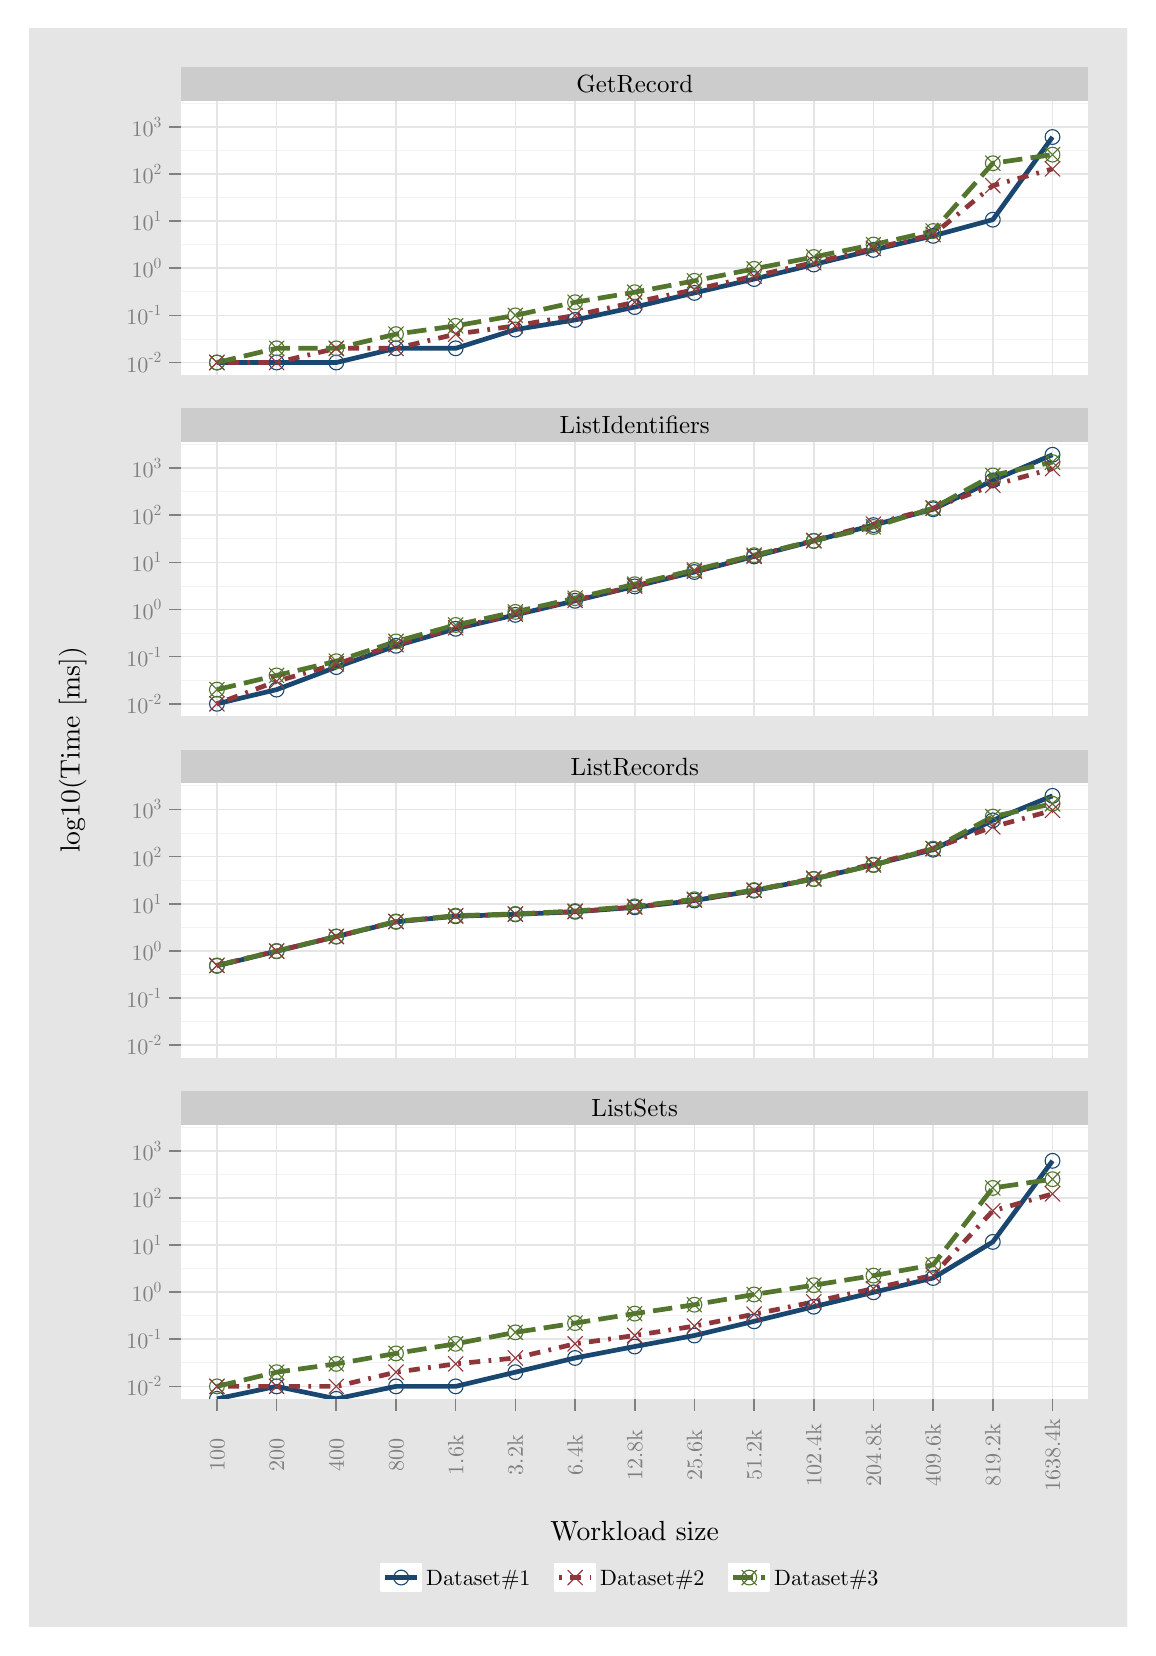
\begin{tikzpicture}[x=1pt,y=1pt]
\definecolor[named]{fillColor}{rgb}{1.00,1.00,1.00}
\path[use as bounding box,fill=fillColor,fill opacity=0.00] (0,0) rectangle (397.48,578.16);
\begin{scope}
\path[clip] (  0.00,  0.00) rectangle (397.48,578.16);
\definecolor[named]{drawColor}{rgb}{1.00,1.00,1.00}
\definecolor[named]{fillColor}{rgb}{0.90,0.90,0.90}

\path[draw=drawColor,line width= 0.6pt,line join=round,line cap=round,fill=fillColor] (  0.00, -0.00) rectangle (397.48,578.16);
\end{scope}
\begin{scope}
\path[clip] ( 55.45,452.66) rectangle (383.26,551.71);
\definecolor[named]{fillColor}{rgb}{1.00,1.00,1.00}

\path[fill=fillColor] ( 55.45,452.66) rectangle (383.26,551.71);
\definecolor[named]{drawColor}{rgb}{0.95,0.95,0.95}

\path[draw=drawColor,line width= 0.3pt,line join=round] ( 55.45,465.68) --
	(383.26,465.68);

\path[draw=drawColor,line width= 0.3pt,line join=round] ( 55.45,482.71) --
	(383.26,482.71);

\path[draw=drawColor,line width= 0.3pt,line join=round] ( 55.45,499.74) --
	(383.26,499.74);

\path[draw=drawColor,line width= 0.3pt,line join=round] ( 55.45,516.77) --
	(383.26,516.77);

\path[draw=drawColor,line width= 0.3pt,line join=round] ( 55.45,533.80) --
	(383.26,533.80);

\path[draw=drawColor,line width= 0.3pt,line join=round] ( 55.45,550.84) --
	(383.26,550.84);
\definecolor[named]{drawColor}{rgb}{0.90,0.90,0.90}

\path[draw=drawColor,line width= 0.6pt,line join=round] ( 55.45,457.16) --
	(383.26,457.16);

\path[draw=drawColor,line width= 0.6pt,line join=round] ( 55.45,474.19) --
	(383.26,474.19);

\path[draw=drawColor,line width= 0.6pt,line join=round] ( 55.45,491.22) --
	(383.26,491.22);

\path[draw=drawColor,line width= 0.6pt,line join=round] ( 55.45,508.26) --
	(383.26,508.26);

\path[draw=drawColor,line width= 0.6pt,line join=round] ( 55.45,525.29) --
	(383.26,525.29);

\path[draw=drawColor,line width= 0.6pt,line join=round] ( 55.45,542.32) --
	(383.26,542.32);

\path[draw=drawColor,line width= 0.6pt,line join=round] ( 68.39,452.66) --
	( 68.39,551.71);

\path[draw=drawColor,line width= 0.6pt,line join=round] ( 89.95,452.66) --
	( 89.95,551.71);

\path[draw=drawColor,line width= 0.6pt,line join=round] (111.52,452.66) --
	(111.52,551.71);

\path[draw=drawColor,line width= 0.6pt,line join=round] (133.09,452.66) --
	(133.09,551.71);

\path[draw=drawColor,line width= 0.6pt,line join=round] (154.65,452.66) --
	(154.65,551.71);

\path[draw=drawColor,line width= 0.6pt,line join=round] (176.22,452.66) --
	(176.22,551.71);

\path[draw=drawColor,line width= 0.6pt,line join=round] (197.79,452.66) --
	(197.79,551.71);

\path[draw=drawColor,line width= 0.6pt,line join=round] (219.35,452.66) --
	(219.35,551.71);

\path[draw=drawColor,line width= 0.6pt,line join=round] (240.92,452.66) --
	(240.92,551.71);

\path[draw=drawColor,line width= 0.6pt,line join=round] (262.49,452.66) --
	(262.49,551.71);

\path[draw=drawColor,line width= 0.6pt,line join=round] (284.05,452.66) --
	(284.05,551.71);

\path[draw=drawColor,line width= 0.6pt,line join=round] (305.62,452.66) --
	(305.62,551.71);

\path[draw=drawColor,line width= 0.6pt,line join=round] (327.19,452.66) --
	(327.19,551.71);

\path[draw=drawColor,line width= 0.6pt,line join=round] (348.75,452.66) --
	(348.75,551.71);

\path[draw=drawColor,line width= 0.6pt,line join=round] (370.32,452.66) --
	(370.32,551.71);
\definecolor[named]{drawColor}{rgb}{0.10,0.28,0.44}

\path[draw=drawColor,line width= 1.7pt,line join=round] ( 68.39,457.16) --
	( 89.95,457.16) --
	(111.52,457.16) --
	(133.09,462.29) --
	(154.65,462.29) --
	(176.22,469.06) --
	(197.79,472.54) --
	(219.35,477.19) --
	(240.92,482.32) --
	(262.49,487.32) --
	(284.05,492.57) --
	(305.62,497.85) --
	(327.19,502.93) --
	(348.75,508.77) --
	(370.32,538.64);
\definecolor[named]{drawColor}{rgb}{0.56,0.21,0.23}

\path[draw=drawColor,line width= 1.7pt,dash pattern=on 1pt off 3pt on 4pt off 3pt ,line join=round] ( 68.39,457.16) --
	( 89.95,457.16) --
	(111.52,462.29) --
	(133.09,462.29) --
	(154.65,467.41) --
	(176.22,470.41) --
	(197.79,474.19) --
	(219.35,478.94) --
	(240.92,483.46) --
	(262.49,488.37) --
	(284.05,493.28) --
	(305.62,498.38) --
	(327.19,503.42) --
	(348.75,521.08) --
	(370.32,527.11);
\definecolor[named]{drawColor}{rgb}{0.33,0.46,0.18}

\path[draw=drawColor,line width= 1.7pt,dash pattern=on 7pt off 3pt ,line join=round] ( 68.39,457.16) --
	( 89.95,462.29) --
	(111.52,462.29) --
	(133.09,467.41) --
	(154.65,470.41) --
	(176.22,474.19) --
	(197.79,478.94) --
	(219.35,482.56) --
	(240.92,486.67) --
	(262.49,491.00) --
	(284.05,495.28) --
	(305.62,499.78) --
	(327.19,504.67) --
	(348.75,529.16) --
	(370.32,532.27);
\definecolor[named]{drawColor}{rgb}{0.10,0.28,0.44}

\path[draw=drawColor,line width= 0.4pt,line join=round,line cap=round] ( 68.39,457.16) circle (  2.67);

\path[draw=drawColor,line width= 0.4pt,line join=round,line cap=round] ( 89.95,457.16) circle (  2.67);

\path[draw=drawColor,line width= 0.4pt,line join=round,line cap=round] (111.52,457.16) circle (  2.67);

\path[draw=drawColor,line width= 0.4pt,line join=round,line cap=round] (133.09,462.29) circle (  2.67);

\path[draw=drawColor,line width= 0.4pt,line join=round,line cap=round] (154.65,462.29) circle (  2.67);

\path[draw=drawColor,line width= 0.4pt,line join=round,line cap=round] (176.22,469.06) circle (  2.67);

\path[draw=drawColor,line width= 0.4pt,line join=round,line cap=round] (197.79,472.54) circle (  2.67);

\path[draw=drawColor,line width= 0.4pt,line join=round,line cap=round] (219.35,477.19) circle (  2.67);

\path[draw=drawColor,line width= 0.4pt,line join=round,line cap=round] (240.92,482.32) circle (  2.67);

\path[draw=drawColor,line width= 0.4pt,line join=round,line cap=round] (262.49,487.32) circle (  2.67);

\path[draw=drawColor,line width= 0.4pt,line join=round,line cap=round] (284.05,492.57) circle (  2.67);

\path[draw=drawColor,line width= 0.4pt,line join=round,line cap=round] (305.62,497.85) circle (  2.67);

\path[draw=drawColor,line width= 0.4pt,line join=round,line cap=round] (327.19,502.93) circle (  2.67);

\path[draw=drawColor,line width= 0.4pt,line join=round,line cap=round] (348.75,508.77) circle (  2.67);

\path[draw=drawColor,line width= 0.4pt,line join=round,line cap=round] (370.32,538.64) circle (  2.67);
\definecolor[named]{drawColor}{rgb}{0.33,0.46,0.18}

\path[draw=drawColor,line width= 0.4pt,line join=round,line cap=round] ( 68.39,457.16) circle (  2.67);

\path[draw=drawColor,line width= 0.4pt,line join=round,line cap=round] ( 65.72,454.49) -- ( 71.06,459.83);

\path[draw=drawColor,line width= 0.4pt,line join=round,line cap=round] ( 65.72,459.83) -- ( 71.06,454.49);

\path[draw=drawColor,line width= 0.4pt,line join=round,line cap=round] ( 89.95,462.29) circle (  2.67);

\path[draw=drawColor,line width= 0.4pt,line join=round,line cap=round] ( 87.29,459.62) -- ( 92.62,464.95);

\path[draw=drawColor,line width= 0.4pt,line join=round,line cap=round] ( 87.29,464.95) -- ( 92.62,459.62);

\path[draw=drawColor,line width= 0.4pt,line join=round,line cap=round] (111.52,462.29) circle (  2.67);

\path[draw=drawColor,line width= 0.4pt,line join=round,line cap=round] (108.85,459.62) -- (114.19,464.95);

\path[draw=drawColor,line width= 0.4pt,line join=round,line cap=round] (108.85,464.95) -- (114.19,459.62);

\path[draw=drawColor,line width= 0.4pt,line join=round,line cap=round] (133.09,467.41) circle (  2.67);

\path[draw=drawColor,line width= 0.4pt,line join=round,line cap=round] (130.42,464.75) -- (135.76,470.08);

\path[draw=drawColor,line width= 0.4pt,line join=round,line cap=round] (130.42,470.08) -- (135.76,464.75);

\path[draw=drawColor,line width= 0.4pt,line join=round,line cap=round] (154.65,470.41) circle (  2.67);

\path[draw=drawColor,line width= 0.4pt,line join=round,line cap=round] (151.99,467.75) -- (157.32,473.08);

\path[draw=drawColor,line width= 0.4pt,line join=round,line cap=round] (151.99,473.08) -- (157.32,467.75);

\path[draw=drawColor,line width= 0.4pt,line join=round,line cap=round] (176.22,474.19) circle (  2.67);

\path[draw=drawColor,line width= 0.4pt,line join=round,line cap=round] (173.55,471.52) -- (178.89,476.86);

\path[draw=drawColor,line width= 0.4pt,line join=round,line cap=round] (173.55,476.86) -- (178.89,471.52);

\path[draw=drawColor,line width= 0.4pt,line join=round,line cap=round] (197.79,478.94) circle (  2.67);

\path[draw=drawColor,line width= 0.4pt,line join=round,line cap=round] (195.12,476.27) -- (200.45,481.61);

\path[draw=drawColor,line width= 0.4pt,line join=round,line cap=round] (195.12,481.61) -- (200.45,476.27);

\path[draw=drawColor,line width= 0.4pt,line join=round,line cap=round] (219.35,482.56) circle (  2.67);

\path[draw=drawColor,line width= 0.4pt,line join=round,line cap=round] (216.69,479.89) -- (222.02,485.23);

\path[draw=drawColor,line width= 0.4pt,line join=round,line cap=round] (216.69,485.23) -- (222.02,479.89);

\path[draw=drawColor,line width= 0.4pt,line join=round,line cap=round] (240.92,486.67) circle (  2.67);

\path[draw=drawColor,line width= 0.4pt,line join=round,line cap=round] (238.25,484.00) -- (243.59,489.33);

\path[draw=drawColor,line width= 0.4pt,line join=round,line cap=round] (238.25,489.33) -- (243.59,484.00);

\path[draw=drawColor,line width= 0.4pt,line join=round,line cap=round] (262.49,491.00) circle (  2.67);

\path[draw=drawColor,line width= 0.4pt,line join=round,line cap=round] (259.82,488.33) -- (265.15,493.67);

\path[draw=drawColor,line width= 0.4pt,line join=round,line cap=round] (259.82,493.67) -- (265.15,488.33);

\path[draw=drawColor,line width= 0.4pt,line join=round,line cap=round] (284.05,495.28) circle (  2.67);

\path[draw=drawColor,line width= 0.4pt,line join=round,line cap=round] (281.39,492.61) -- (286.72,497.95);

\path[draw=drawColor,line width= 0.4pt,line join=round,line cap=round] (281.39,497.95) -- (286.72,492.61);

\path[draw=drawColor,line width= 0.4pt,line join=round,line cap=round] (305.62,499.78) circle (  2.67);

\path[draw=drawColor,line width= 0.4pt,line join=round,line cap=round] (302.95,497.11) -- (308.29,502.45);

\path[draw=drawColor,line width= 0.4pt,line join=round,line cap=round] (302.95,502.45) -- (308.29,497.11);

\path[draw=drawColor,line width= 0.4pt,line join=round,line cap=round] (327.19,504.67) circle (  2.67);

\path[draw=drawColor,line width= 0.4pt,line join=round,line cap=round] (324.52,502.00) -- (329.85,507.34);

\path[draw=drawColor,line width= 0.4pt,line join=round,line cap=round] (324.52,507.34) -- (329.85,502.00);

\path[draw=drawColor,line width= 0.4pt,line join=round,line cap=round] (348.75,529.16) circle (  2.67);

\path[draw=drawColor,line width= 0.4pt,line join=round,line cap=round] (346.08,526.50) -- (351.42,531.83);

\path[draw=drawColor,line width= 0.4pt,line join=round,line cap=round] (346.08,531.83) -- (351.42,526.50);

\path[draw=drawColor,line width= 0.4pt,line join=round,line cap=round] (370.32,532.27) circle (  2.67);

\path[draw=drawColor,line width= 0.4pt,line join=round,line cap=round] (367.65,529.61) -- (372.99,534.94);

\path[draw=drawColor,line width= 0.4pt,line join=round,line cap=round] (367.65,534.94) -- (372.99,529.61);
\definecolor[named]{drawColor}{rgb}{0.56,0.21,0.23}

\path[draw=drawColor,line width= 0.4pt,line join=round,line cap=round,fill=fillColor] ( 65.72,454.49) -- ( 71.06,459.83);

\path[draw=drawColor,line width= 0.4pt,line join=round,line cap=round,fill=fillColor] ( 65.72,459.83) -- ( 71.06,454.49);

\path[draw=drawColor,line width= 0.4pt,line join=round,line cap=round,fill=fillColor] ( 87.29,454.49) -- ( 92.62,459.83);

\path[draw=drawColor,line width= 0.4pt,line join=round,line cap=round,fill=fillColor] ( 87.29,459.83) -- ( 92.62,454.49);

\path[draw=drawColor,line width= 0.4pt,line join=round,line cap=round,fill=fillColor] (108.85,459.62) -- (114.19,464.95);

\path[draw=drawColor,line width= 0.4pt,line join=round,line cap=round,fill=fillColor] (108.85,464.95) -- (114.19,459.62);

\path[draw=drawColor,line width= 0.4pt,line join=round,line cap=round,fill=fillColor] (130.42,459.62) -- (135.76,464.95);

\path[draw=drawColor,line width= 0.4pt,line join=round,line cap=round,fill=fillColor] (130.42,464.95) -- (135.76,459.62);

\path[draw=drawColor,line width= 0.4pt,line join=round,line cap=round,fill=fillColor] (151.99,464.75) -- (157.32,470.08);

\path[draw=drawColor,line width= 0.4pt,line join=round,line cap=round,fill=fillColor] (151.99,470.08) -- (157.32,464.75);

\path[draw=drawColor,line width= 0.4pt,line join=round,line cap=round,fill=fillColor] (173.55,467.75) -- (178.89,473.08);

\path[draw=drawColor,line width= 0.4pt,line join=round,line cap=round,fill=fillColor] (173.55,473.08) -- (178.89,467.75);

\path[draw=drawColor,line width= 0.4pt,line join=round,line cap=round,fill=fillColor] (195.12,471.52) -- (200.45,476.86);

\path[draw=drawColor,line width= 0.4pt,line join=round,line cap=round,fill=fillColor] (195.12,476.86) -- (200.45,471.52);

\path[draw=drawColor,line width= 0.4pt,line join=round,line cap=round,fill=fillColor] (216.69,476.27) -- (222.02,481.61);

\path[draw=drawColor,line width= 0.4pt,line join=round,line cap=round,fill=fillColor] (216.69,481.61) -- (222.02,476.27);

\path[draw=drawColor,line width= 0.4pt,line join=round,line cap=round,fill=fillColor] (238.25,480.79) -- (243.59,486.13);

\path[draw=drawColor,line width= 0.4pt,line join=round,line cap=round,fill=fillColor] (238.25,486.13) -- (243.59,480.79);

\path[draw=drawColor,line width= 0.4pt,line join=round,line cap=round,fill=fillColor] (259.82,485.70) -- (265.15,491.04);

\path[draw=drawColor,line width= 0.4pt,line join=round,line cap=round,fill=fillColor] (259.82,491.04) -- (265.15,485.70);

\path[draw=drawColor,line width= 0.4pt,line join=round,line cap=round,fill=fillColor] (281.39,490.61) -- (286.72,495.94);

\path[draw=drawColor,line width= 0.4pt,line join=round,line cap=round,fill=fillColor] (281.39,495.94) -- (286.72,490.61);

\path[draw=drawColor,line width= 0.4pt,line join=round,line cap=round,fill=fillColor] (302.95,495.71) -- (308.29,501.04);

\path[draw=drawColor,line width= 0.4pt,line join=round,line cap=round,fill=fillColor] (302.95,501.04) -- (308.29,495.71);

\path[draw=drawColor,line width= 0.4pt,line join=round,line cap=round,fill=fillColor] (324.52,500.75) -- (329.85,506.09);

\path[draw=drawColor,line width= 0.4pt,line join=round,line cap=round,fill=fillColor] (324.52,506.09) -- (329.85,500.75);

\path[draw=drawColor,line width= 0.4pt,line join=round,line cap=round,fill=fillColor] (346.08,518.42) -- (351.42,523.75);

\path[draw=drawColor,line width= 0.4pt,line join=round,line cap=round,fill=fillColor] (346.08,523.75) -- (351.42,518.42);

\path[draw=drawColor,line width= 0.4pt,line join=round,line cap=round,fill=fillColor] (367.65,524.45) -- (372.99,529.78);

\path[draw=drawColor,line width= 0.4pt,line join=round,line cap=round,fill=fillColor] (367.65,529.78) -- (372.99,524.45);
\end{scope}
\begin{scope}
\path[clip] ( 55.45,329.33) rectangle (383.26,428.39);
\definecolor[named]{fillColor}{rgb}{1.00,1.00,1.00}

\path[fill=fillColor] ( 55.45,329.33) rectangle (383.26,428.39);
\definecolor[named]{drawColor}{rgb}{0.95,0.95,0.95}

\path[draw=drawColor,line width= 0.3pt,line join=round] ( 55.45,342.35) --
	(383.26,342.35);

\path[draw=drawColor,line width= 0.3pt,line join=round] ( 55.45,359.39) --
	(383.26,359.39);

\path[draw=drawColor,line width= 0.3pt,line join=round] ( 55.45,376.42) --
	(383.26,376.42);

\path[draw=drawColor,line width= 0.3pt,line join=round] ( 55.45,393.45) --
	(383.26,393.45);

\path[draw=drawColor,line width= 0.3pt,line join=round] ( 55.45,410.48) --
	(383.26,410.48);

\path[draw=drawColor,line width= 0.3pt,line join=round] ( 55.45,427.51) --
	(383.26,427.51);
\definecolor[named]{drawColor}{rgb}{0.90,0.90,0.90}

\path[draw=drawColor,line width= 0.6pt,line join=round] ( 55.45,333.84) --
	(383.26,333.84);

\path[draw=drawColor,line width= 0.6pt,line join=round] ( 55.45,350.87) --
	(383.26,350.87);

\path[draw=drawColor,line width= 0.6pt,line join=round] ( 55.45,367.90) --
	(383.26,367.90);

\path[draw=drawColor,line width= 0.6pt,line join=round] ( 55.45,384.93) --
	(383.26,384.93);

\path[draw=drawColor,line width= 0.6pt,line join=round] ( 55.45,401.97) --
	(383.26,401.97);

\path[draw=drawColor,line width= 0.6pt,line join=round] ( 55.45,419.00) --
	(383.26,419.00);

\path[draw=drawColor,line width= 0.6pt,line join=round] ( 68.39,329.33) --
	( 68.39,428.39);

\path[draw=drawColor,line width= 0.6pt,line join=round] ( 89.95,329.33) --
	( 89.95,428.39);

\path[draw=drawColor,line width= 0.6pt,line join=round] (111.52,329.33) --
	(111.52,428.39);

\path[draw=drawColor,line width= 0.6pt,line join=round] (133.09,329.33) --
	(133.09,428.39);

\path[draw=drawColor,line width= 0.6pt,line join=round] (154.65,329.33) --
	(154.65,428.39);

\path[draw=drawColor,line width= 0.6pt,line join=round] (176.22,329.33) --
	(176.22,428.39);

\path[draw=drawColor,line width= 0.6pt,line join=round] (197.79,329.33) --
	(197.79,428.39);

\path[draw=drawColor,line width= 0.6pt,line join=round] (219.35,329.33) --
	(219.35,428.39);

\path[draw=drawColor,line width= 0.6pt,line join=round] (240.92,329.33) --
	(240.92,428.39);

\path[draw=drawColor,line width= 0.6pt,line join=round] (262.49,329.33) --
	(262.49,428.39);

\path[draw=drawColor,line width= 0.6pt,line join=round] (284.05,329.33) --
	(284.05,428.39);

\path[draw=drawColor,line width= 0.6pt,line join=round] (305.62,329.33) --
	(305.62,428.39);

\path[draw=drawColor,line width= 0.6pt,line join=round] (327.19,329.33) --
	(327.19,428.39);

\path[draw=drawColor,line width= 0.6pt,line join=round] (348.75,329.33) --
	(348.75,428.39);

\path[draw=drawColor,line width= 0.6pt,line join=round] (370.32,329.33) --
	(370.32,428.39);
\definecolor[named]{drawColor}{rgb}{0.10,0.28,0.44}

\path[draw=drawColor,line width= 1.7pt,line join=round] ( 68.39,333.84) --
	( 89.95,338.96) --
	(111.52,347.09) --
	(133.09,354.79) --
	(154.65,360.94) --
	(176.22,365.97) --
	(197.79,371.05) --
	(219.35,376.25) --
	(240.92,381.46) --
	(262.49,387.09) --
	(284.05,392.67) --
	(305.62,398.41) --
	(327.19,404.13) --
	(348.75,414.55) --
	(370.32,423.83);
\definecolor[named]{drawColor}{rgb}{0.56,0.21,0.23}

\path[draw=drawColor,line width= 1.7pt,dash pattern=on 1pt off 3pt on 4pt off 3pt ,line join=round] ( 68.39,333.84) --
	( 89.95,341.96) --
	(111.52,348.23) --
	(133.09,355.22) --
	(154.65,361.31) --
	(176.22,366.25) --
	(197.79,371.24) --
	(219.35,376.41) --
	(240.92,381.71) --
	(262.49,387.13) --
	(284.05,392.90) --
	(305.62,398.77) --
	(327.19,404.53) --
	(348.75,412.80) --
	(370.32,418.80);
\definecolor[named]{drawColor}{rgb}{0.33,0.46,0.18}

\path[draw=drawColor,line width= 1.7pt,dash pattern=on 7pt off 3pt ,line join=round] ( 68.39,338.96) --
	( 89.95,344.09) --
	(111.52,349.22) --
	(133.09,356.36) --
	(154.65,362.32) --
	(176.22,367.04) --
	(197.79,372.00) --
	(219.35,377.04) --
	(240.92,382.19) --
	(262.49,387.54) --
	(284.05,392.75) --
	(305.62,397.74) --
	(327.19,404.56) --
	(348.75,416.36) --
	(370.32,421.17);
\definecolor[named]{drawColor}{rgb}{0.10,0.28,0.44}

\path[draw=drawColor,line width= 0.4pt,line join=round,line cap=round] ( 68.39,333.84) circle (  2.67);

\path[draw=drawColor,line width= 0.4pt,line join=round,line cap=round] ( 89.95,338.96) circle (  2.67);

\path[draw=drawColor,line width= 0.4pt,line join=round,line cap=round] (111.52,347.09) circle (  2.67);

\path[draw=drawColor,line width= 0.4pt,line join=round,line cap=round] (133.09,354.79) circle (  2.67);

\path[draw=drawColor,line width= 0.4pt,line join=round,line cap=round] (154.65,360.94) circle (  2.67);

\path[draw=drawColor,line width= 0.4pt,line join=round,line cap=round] (176.22,365.97) circle (  2.67);

\path[draw=drawColor,line width= 0.4pt,line join=round,line cap=round] (197.79,371.05) circle (  2.67);

\path[draw=drawColor,line width= 0.4pt,line join=round,line cap=round] (219.35,376.25) circle (  2.67);

\path[draw=drawColor,line width= 0.4pt,line join=round,line cap=round] (240.92,381.46) circle (  2.67);

\path[draw=drawColor,line width= 0.4pt,line join=round,line cap=round] (262.49,387.09) circle (  2.67);

\path[draw=drawColor,line width= 0.4pt,line join=round,line cap=round] (284.05,392.67) circle (  2.67);

\path[draw=drawColor,line width= 0.4pt,line join=round,line cap=round] (305.62,398.41) circle (  2.67);

\path[draw=drawColor,line width= 0.4pt,line join=round,line cap=round] (327.19,404.13) circle (  2.67);

\path[draw=drawColor,line width= 0.4pt,line join=round,line cap=round] (348.75,414.55) circle (  2.67);

\path[draw=drawColor,line width= 0.4pt,line join=round,line cap=round] (370.32,423.83) circle (  2.67);
\definecolor[named]{drawColor}{rgb}{0.33,0.46,0.18}

\path[draw=drawColor,line width= 0.4pt,line join=round,line cap=round] ( 68.39,338.96) circle (  2.67);

\path[draw=drawColor,line width= 0.4pt,line join=round,line cap=round] ( 65.72,336.30) -- ( 71.06,341.63);

\path[draw=drawColor,line width= 0.4pt,line join=round,line cap=round] ( 65.72,341.63) -- ( 71.06,336.30);

\path[draw=drawColor,line width= 0.4pt,line join=round,line cap=round] ( 89.95,344.09) circle (  2.67);

\path[draw=drawColor,line width= 0.4pt,line join=round,line cap=round] ( 87.29,341.42) -- ( 92.62,346.76);

\path[draw=drawColor,line width= 0.4pt,line join=round,line cap=round] ( 87.29,346.76) -- ( 92.62,341.42);

\path[draw=drawColor,line width= 0.4pt,line join=round,line cap=round] (111.52,349.22) circle (  2.67);

\path[draw=drawColor,line width= 0.4pt,line join=round,line cap=round] (108.85,346.55) -- (114.19,351.89);

\path[draw=drawColor,line width= 0.4pt,line join=round,line cap=round] (108.85,351.89) -- (114.19,346.55);

\path[draw=drawColor,line width= 0.4pt,line join=round,line cap=round] (133.09,356.36) circle (  2.67);

\path[draw=drawColor,line width= 0.4pt,line join=round,line cap=round] (130.42,353.69) -- (135.76,359.02);

\path[draw=drawColor,line width= 0.4pt,line join=round,line cap=round] (130.42,359.02) -- (135.76,353.69);

\path[draw=drawColor,line width= 0.4pt,line join=round,line cap=round] (154.65,362.32) circle (  2.67);

\path[draw=drawColor,line width= 0.4pt,line join=round,line cap=round] (151.99,359.65) -- (157.32,364.98);

\path[draw=drawColor,line width= 0.4pt,line join=round,line cap=round] (151.99,364.98) -- (157.32,359.65);

\path[draw=drawColor,line width= 0.4pt,line join=round,line cap=round] (176.22,367.04) circle (  2.67);

\path[draw=drawColor,line width= 0.4pt,line join=round,line cap=round] (173.55,364.37) -- (178.89,369.71);

\path[draw=drawColor,line width= 0.4pt,line join=round,line cap=round] (173.55,369.71) -- (178.89,364.37);

\path[draw=drawColor,line width= 0.4pt,line join=round,line cap=round] (197.79,372.00) circle (  2.67);

\path[draw=drawColor,line width= 0.4pt,line join=round,line cap=round] (195.12,369.33) -- (200.45,374.67);

\path[draw=drawColor,line width= 0.4pt,line join=round,line cap=round] (195.12,374.67) -- (200.45,369.33);

\path[draw=drawColor,line width= 0.4pt,line join=round,line cap=round] (219.35,377.04) circle (  2.67);

\path[draw=drawColor,line width= 0.4pt,line join=round,line cap=round] (216.69,374.37) -- (222.02,379.71);

\path[draw=drawColor,line width= 0.4pt,line join=round,line cap=round] (216.69,379.71) -- (222.02,374.37);

\path[draw=drawColor,line width= 0.4pt,line join=round,line cap=round] (240.92,382.19) circle (  2.67);

\path[draw=drawColor,line width= 0.4pt,line join=round,line cap=round] (238.25,379.52) -- (243.59,384.86);

\path[draw=drawColor,line width= 0.4pt,line join=round,line cap=round] (238.25,384.86) -- (243.59,379.52);

\path[draw=drawColor,line width= 0.4pt,line join=round,line cap=round] (262.49,387.54) circle (  2.67);

\path[draw=drawColor,line width= 0.4pt,line join=round,line cap=round] (259.82,384.88) -- (265.15,390.21);

\path[draw=drawColor,line width= 0.4pt,line join=round,line cap=round] (259.82,390.21) -- (265.15,384.88);

\path[draw=drawColor,line width= 0.4pt,line join=round,line cap=round] (284.05,392.75) circle (  2.67);

\path[draw=drawColor,line width= 0.4pt,line join=round,line cap=round] (281.39,390.08) -- (286.72,395.42);

\path[draw=drawColor,line width= 0.4pt,line join=round,line cap=round] (281.39,395.42) -- (286.72,390.08);

\path[draw=drawColor,line width= 0.4pt,line join=round,line cap=round] (305.62,397.74) circle (  2.67);

\path[draw=drawColor,line width= 0.4pt,line join=round,line cap=round] (302.95,395.08) -- (308.29,400.41);

\path[draw=drawColor,line width= 0.4pt,line join=round,line cap=round] (302.95,400.41) -- (308.29,395.08);

\path[draw=drawColor,line width= 0.4pt,line join=round,line cap=round] (327.19,404.56) circle (  2.67);

\path[draw=drawColor,line width= 0.4pt,line join=round,line cap=round] (324.52,401.89) -- (329.85,407.22);

\path[draw=drawColor,line width= 0.4pt,line join=round,line cap=round] (324.52,407.22) -- (329.85,401.89);

\path[draw=drawColor,line width= 0.4pt,line join=round,line cap=round] (348.75,416.36) circle (  2.67);

\path[draw=drawColor,line width= 0.4pt,line join=round,line cap=round] (346.08,413.69) -- (351.42,419.03);

\path[draw=drawColor,line width= 0.4pt,line join=round,line cap=round] (346.08,419.03) -- (351.42,413.69);

\path[draw=drawColor,line width= 0.4pt,line join=round,line cap=round] (370.32,421.17) circle (  2.67);

\path[draw=drawColor,line width= 0.4pt,line join=round,line cap=round] (367.65,418.51) -- (372.99,423.84);

\path[draw=drawColor,line width= 0.4pt,line join=round,line cap=round] (367.65,423.84) -- (372.99,418.51);
\definecolor[named]{drawColor}{rgb}{0.56,0.21,0.23}

\path[draw=drawColor,line width= 0.4pt,line join=round,line cap=round,fill=fillColor] ( 65.72,331.17) -- ( 71.06,336.50);

\path[draw=drawColor,line width= 0.4pt,line join=round,line cap=round,fill=fillColor] ( 65.72,336.50) -- ( 71.06,331.17);

\path[draw=drawColor,line width= 0.4pt,line join=round,line cap=round,fill=fillColor] ( 87.29,339.30) -- ( 92.62,344.63);

\path[draw=drawColor,line width= 0.4pt,line join=round,line cap=round,fill=fillColor] ( 87.29,344.63) -- ( 92.62,339.30);

\path[draw=drawColor,line width= 0.4pt,line join=round,line cap=round,fill=fillColor] (108.85,345.56) -- (114.19,350.90);

\path[draw=drawColor,line width= 0.4pt,line join=round,line cap=round,fill=fillColor] (108.85,350.90) -- (114.19,345.56);

\path[draw=drawColor,line width= 0.4pt,line join=round,line cap=round,fill=fillColor] (130.42,352.55) -- (135.76,357.88);

\path[draw=drawColor,line width= 0.4pt,line join=round,line cap=round,fill=fillColor] (130.42,357.88) -- (135.76,352.55);

\path[draw=drawColor,line width= 0.4pt,line join=round,line cap=round,fill=fillColor] (151.99,358.64) -- (157.32,363.97);

\path[draw=drawColor,line width= 0.4pt,line join=round,line cap=round,fill=fillColor] (151.99,363.97) -- (157.32,358.64);

\path[draw=drawColor,line width= 0.4pt,line join=round,line cap=round,fill=fillColor] (173.55,363.58) -- (178.89,368.92);

\path[draw=drawColor,line width= 0.4pt,line join=round,line cap=round,fill=fillColor] (173.55,368.92) -- (178.89,363.58);

\path[draw=drawColor,line width= 0.4pt,line join=round,line cap=round,fill=fillColor] (195.12,368.57) -- (200.45,373.91);

\path[draw=drawColor,line width= 0.4pt,line join=round,line cap=round,fill=fillColor] (195.12,373.91) -- (200.45,368.57);

\path[draw=drawColor,line width= 0.4pt,line join=round,line cap=round,fill=fillColor] (216.69,373.74) -- (222.02,379.08);

\path[draw=drawColor,line width= 0.4pt,line join=round,line cap=round,fill=fillColor] (216.69,379.08) -- (222.02,373.74);

\path[draw=drawColor,line width= 0.4pt,line join=round,line cap=round,fill=fillColor] (238.25,379.05) -- (243.59,384.38);

\path[draw=drawColor,line width= 0.4pt,line join=round,line cap=round,fill=fillColor] (238.25,384.38) -- (243.59,379.05);

\path[draw=drawColor,line width= 0.4pt,line join=round,line cap=round,fill=fillColor] (259.82,384.46) -- (265.15,389.79);

\path[draw=drawColor,line width= 0.4pt,line join=round,line cap=round,fill=fillColor] (259.82,389.79) -- (265.15,384.46);

\path[draw=drawColor,line width= 0.4pt,line join=round,line cap=round,fill=fillColor] (281.39,390.24) -- (286.72,395.57);

\path[draw=drawColor,line width= 0.4pt,line join=round,line cap=round,fill=fillColor] (281.39,395.57) -- (286.72,390.24);

\path[draw=drawColor,line width= 0.4pt,line join=round,line cap=round,fill=fillColor] (302.95,396.10) -- (308.29,401.44);

\path[draw=drawColor,line width= 0.4pt,line join=round,line cap=round,fill=fillColor] (302.95,401.44) -- (308.29,396.10);

\path[draw=drawColor,line width= 0.4pt,line join=round,line cap=round,fill=fillColor] (324.52,401.86) -- (329.85,407.20);

\path[draw=drawColor,line width= 0.4pt,line join=round,line cap=round,fill=fillColor] (324.52,407.20) -- (329.85,401.86);

\path[draw=drawColor,line width= 0.4pt,line join=round,line cap=round,fill=fillColor] (346.08,410.13) -- (351.42,415.47);

\path[draw=drawColor,line width= 0.4pt,line join=round,line cap=round,fill=fillColor] (346.08,415.47) -- (351.42,410.13);

\path[draw=drawColor,line width= 0.4pt,line join=round,line cap=round,fill=fillColor] (367.65,416.13) -- (372.99,421.47);

\path[draw=drawColor,line width= 0.4pt,line join=round,line cap=round,fill=fillColor] (367.65,421.47) -- (372.99,416.13);
\end{scope}
\begin{scope}
\path[clip] ( 55.45,206.01) rectangle (383.26,305.07);
\definecolor[named]{fillColor}{rgb}{1.00,1.00,1.00}

\path[fill=fillColor] ( 55.45,206.01) rectangle (383.26,305.07);
\definecolor[named]{drawColor}{rgb}{0.95,0.95,0.95}

\path[draw=drawColor,line width= 0.3pt,line join=round] ( 55.45,219.03) --
	(383.26,219.03);

\path[draw=drawColor,line width= 0.3pt,line join=round] ( 55.45,236.06) --
	(383.26,236.06);

\path[draw=drawColor,line width= 0.3pt,line join=round] ( 55.45,253.10) --
	(383.26,253.10);

\path[draw=drawColor,line width= 0.3pt,line join=round] ( 55.45,270.13) --
	(383.26,270.13);

\path[draw=drawColor,line width= 0.3pt,line join=round] ( 55.45,287.16) --
	(383.26,287.16);

\path[draw=drawColor,line width= 0.3pt,line join=round] ( 55.45,304.19) --
	(383.26,304.19);
\definecolor[named]{drawColor}{rgb}{0.90,0.90,0.90}

\path[draw=drawColor,line width= 0.6pt,line join=round] ( 55.45,210.52) --
	(383.26,210.52);

\path[draw=drawColor,line width= 0.6pt,line join=round] ( 55.45,227.55) --
	(383.26,227.55);

\path[draw=drawColor,line width= 0.6pt,line join=round] ( 55.45,244.58) --
	(383.26,244.58);

\path[draw=drawColor,line width= 0.6pt,line join=round] ( 55.45,261.61) --
	(383.26,261.61);

\path[draw=drawColor,line width= 0.6pt,line join=round] ( 55.45,278.64) --
	(383.26,278.64);

\path[draw=drawColor,line width= 0.6pt,line join=round] ( 55.45,295.68) --
	(383.26,295.68);

\path[draw=drawColor,line width= 0.6pt,line join=round] ( 68.39,206.01) --
	( 68.39,305.07);

\path[draw=drawColor,line width= 0.6pt,line join=round] ( 89.95,206.01) --
	( 89.95,305.07);

\path[draw=drawColor,line width= 0.6pt,line join=round] (111.52,206.01) --
	(111.52,305.07);

\path[draw=drawColor,line width= 0.6pt,line join=round] (133.09,206.01) --
	(133.09,305.07);

\path[draw=drawColor,line width= 0.6pt,line join=round] (154.65,206.01) --
	(154.65,305.07);

\path[draw=drawColor,line width= 0.6pt,line join=round] (176.22,206.01) --
	(176.22,305.07);

\path[draw=drawColor,line width= 0.6pt,line join=round] (197.79,206.01) --
	(197.79,305.07);

\path[draw=drawColor,line width= 0.6pt,line join=round] (219.35,206.01) --
	(219.35,305.07);

\path[draw=drawColor,line width= 0.6pt,line join=round] (240.92,206.01) --
	(240.92,305.07);

\path[draw=drawColor,line width= 0.6pt,line join=round] (262.49,206.01) --
	(262.49,305.07);

\path[draw=drawColor,line width= 0.6pt,line join=round] (284.05,206.01) --
	(284.05,305.07);

\path[draw=drawColor,line width= 0.6pt,line join=round] (305.62,206.01) --
	(305.62,305.07);

\path[draw=drawColor,line width= 0.6pt,line join=round] (327.19,206.01) --
	(327.19,305.07);

\path[draw=drawColor,line width= 0.6pt,line join=round] (348.75,206.01) --
	(348.75,305.07);

\path[draw=drawColor,line width= 0.6pt,line join=round] (370.32,206.01) --
	(370.32,305.07);
\definecolor[named]{drawColor}{rgb}{0.10,0.28,0.44}

\path[draw=drawColor,line width= 1.7pt,line join=round] ( 68.39,239.15) --
	( 89.95,244.43) --
	(111.52,249.71) --
	(133.09,255.05) --
	(154.65,257.07) --
	(176.22,257.76) --
	(197.79,258.68) --
	(219.35,260.30) --
	(240.92,262.76) --
	(262.49,266.32) --
	(284.05,270.55) --
	(305.62,275.68) --
	(327.19,281.12) --
	(348.75,291.73) --
	(370.32,300.57);
\definecolor[named]{drawColor}{rgb}{0.56,0.21,0.23}

\path[draw=drawColor,line width= 1.7pt,dash pattern=on 1pt off 3pt on 4pt off 3pt ,line join=round] ( 68.39,239.30) --
	( 89.95,244.51) --
	(111.52,249.74) --
	(133.09,255.14) --
	(154.65,257.15) --
	(176.22,257.80) --
	(197.79,258.74) --
	(219.35,260.40) --
	(240.92,262.94) --
	(262.49,266.40) --
	(284.05,270.80) --
	(305.62,275.99) --
	(327.19,281.53) --
	(348.75,289.36) --
	(370.32,295.31);
\definecolor[named]{drawColor}{rgb}{0.33,0.46,0.18}

\path[draw=drawColor,line width= 1.7pt,dash pattern=on 7pt off 3pt ,line join=round] ( 68.39,239.30) --
	( 89.95,244.51) --
	(111.52,249.78) --
	(133.09,255.19) --
	(154.65,257.28) --
	(176.22,257.91) --
	(197.79,258.95) --
	(219.35,260.66) --
	(240.92,263.22) --
	(262.49,266.52) --
	(284.05,270.51) --
	(305.62,275.55) --
	(327.19,281.50) --
	(348.75,293.08) --
	(370.32,297.72);
\definecolor[named]{drawColor}{rgb}{0.10,0.28,0.44}

\path[draw=drawColor,line width= 0.4pt,line join=round,line cap=round] ( 68.39,239.15) circle (  2.67);

\path[draw=drawColor,line width= 0.4pt,line join=round,line cap=round] ( 89.95,244.43) circle (  2.67);

\path[draw=drawColor,line width= 0.4pt,line join=round,line cap=round] (111.52,249.71) circle (  2.67);

\path[draw=drawColor,line width= 0.4pt,line join=round,line cap=round] (133.09,255.05) circle (  2.67);

\path[draw=drawColor,line width= 0.4pt,line join=round,line cap=round] (154.65,257.07) circle (  2.67);

\path[draw=drawColor,line width= 0.4pt,line join=round,line cap=round] (176.22,257.76) circle (  2.67);

\path[draw=drawColor,line width= 0.4pt,line join=round,line cap=round] (197.79,258.68) circle (  2.67);

\path[draw=drawColor,line width= 0.4pt,line join=round,line cap=round] (219.35,260.30) circle (  2.67);

\path[draw=drawColor,line width= 0.4pt,line join=round,line cap=round] (240.92,262.76) circle (  2.67);

\path[draw=drawColor,line width= 0.4pt,line join=round,line cap=round] (262.49,266.32) circle (  2.67);

\path[draw=drawColor,line width= 0.4pt,line join=round,line cap=round] (284.05,270.55) circle (  2.67);

\path[draw=drawColor,line width= 0.4pt,line join=round,line cap=round] (305.62,275.68) circle (  2.67);

\path[draw=drawColor,line width= 0.4pt,line join=round,line cap=round] (327.19,281.12) circle (  2.67);

\path[draw=drawColor,line width= 0.4pt,line join=round,line cap=round] (348.75,291.73) circle (  2.67);

\path[draw=drawColor,line width= 0.4pt,line join=round,line cap=round] (370.32,300.57) circle (  2.67);
\definecolor[named]{drawColor}{rgb}{0.33,0.46,0.18}

\path[draw=drawColor,line width= 0.4pt,line join=round,line cap=round] ( 68.39,239.30) circle (  2.67);

\path[draw=drawColor,line width= 0.4pt,line join=round,line cap=round] ( 65.72,236.64) -- ( 71.06,241.97);

\path[draw=drawColor,line width= 0.4pt,line join=round,line cap=round] ( 65.72,241.97) -- ( 71.06,236.64);

\path[draw=drawColor,line width= 0.4pt,line join=round,line cap=round] ( 89.95,244.51) circle (  2.67);

\path[draw=drawColor,line width= 0.4pt,line join=round,line cap=round] ( 87.29,241.84) -- ( 92.62,247.17);

\path[draw=drawColor,line width= 0.4pt,line join=round,line cap=round] ( 87.29,247.17) -- ( 92.62,241.84);

\path[draw=drawColor,line width= 0.4pt,line join=round,line cap=round] (111.52,249.78) circle (  2.67);

\path[draw=drawColor,line width= 0.4pt,line join=round,line cap=round] (108.85,247.11) -- (114.19,252.45);

\path[draw=drawColor,line width= 0.4pt,line join=round,line cap=round] (108.85,252.45) -- (114.19,247.11);

\path[draw=drawColor,line width= 0.4pt,line join=round,line cap=round] (133.09,255.19) circle (  2.67);

\path[draw=drawColor,line width= 0.4pt,line join=round,line cap=round] (130.42,252.53) -- (135.76,257.86);

\path[draw=drawColor,line width= 0.4pt,line join=round,line cap=round] (130.42,257.86) -- (135.76,252.53);

\path[draw=drawColor,line width= 0.4pt,line join=round,line cap=round] (154.65,257.28) circle (  2.67);

\path[draw=drawColor,line width= 0.4pt,line join=round,line cap=round] (151.99,254.62) -- (157.32,259.95);

\path[draw=drawColor,line width= 0.4pt,line join=round,line cap=round] (151.99,259.95) -- (157.32,254.62);

\path[draw=drawColor,line width= 0.4pt,line join=round,line cap=round] (176.22,257.91) circle (  2.67);

\path[draw=drawColor,line width= 0.4pt,line join=round,line cap=round] (173.55,255.24) -- (178.89,260.57);

\path[draw=drawColor,line width= 0.4pt,line join=round,line cap=round] (173.55,260.57) -- (178.89,255.24);

\path[draw=drawColor,line width= 0.4pt,line join=round,line cap=round] (197.79,258.95) circle (  2.67);

\path[draw=drawColor,line width= 0.4pt,line join=round,line cap=round] (195.12,256.28) -- (200.45,261.62);

\path[draw=drawColor,line width= 0.4pt,line join=round,line cap=round] (195.12,261.62) -- (200.45,256.28);

\path[draw=drawColor,line width= 0.4pt,line join=round,line cap=round] (219.35,260.66) circle (  2.67);

\path[draw=drawColor,line width= 0.4pt,line join=round,line cap=round] (216.69,257.99) -- (222.02,263.32);

\path[draw=drawColor,line width= 0.4pt,line join=round,line cap=round] (216.69,263.32) -- (222.02,257.99);

\path[draw=drawColor,line width= 0.4pt,line join=round,line cap=round] (240.92,263.22) circle (  2.67);

\path[draw=drawColor,line width= 0.4pt,line join=round,line cap=round] (238.25,260.55) -- (243.59,265.89);

\path[draw=drawColor,line width= 0.4pt,line join=round,line cap=round] (238.25,265.89) -- (243.59,260.55);

\path[draw=drawColor,line width= 0.4pt,line join=round,line cap=round] (262.49,266.52) circle (  2.67);

\path[draw=drawColor,line width= 0.4pt,line join=round,line cap=round] (259.82,263.86) -- (265.15,269.19);

\path[draw=drawColor,line width= 0.4pt,line join=round,line cap=round] (259.82,269.19) -- (265.15,263.86);

\path[draw=drawColor,line width= 0.4pt,line join=round,line cap=round] (284.05,270.51) circle (  2.67);

\path[draw=drawColor,line width= 0.4pt,line join=round,line cap=round] (281.39,267.84) -- (286.72,273.18);

\path[draw=drawColor,line width= 0.4pt,line join=round,line cap=round] (281.39,273.18) -- (286.72,267.84);

\path[draw=drawColor,line width= 0.4pt,line join=round,line cap=round] (305.62,275.55) circle (  2.67);

\path[draw=drawColor,line width= 0.4pt,line join=round,line cap=round] (302.95,272.88) -- (308.29,278.21);

\path[draw=drawColor,line width= 0.4pt,line join=round,line cap=round] (302.95,278.21) -- (308.29,272.88);

\path[draw=drawColor,line width= 0.4pt,line join=round,line cap=round] (327.19,281.50) circle (  2.67);

\path[draw=drawColor,line width= 0.4pt,line join=round,line cap=round] (324.52,278.84) -- (329.85,284.17);

\path[draw=drawColor,line width= 0.4pt,line join=round,line cap=round] (324.52,284.17) -- (329.85,278.84);

\path[draw=drawColor,line width= 0.4pt,line join=round,line cap=round] (348.75,293.08) circle (  2.67);

\path[draw=drawColor,line width= 0.4pt,line join=round,line cap=round] (346.08,290.41) -- (351.42,295.75);

\path[draw=drawColor,line width= 0.4pt,line join=round,line cap=round] (346.08,295.75) -- (351.42,290.41);

\path[draw=drawColor,line width= 0.4pt,line join=round,line cap=round] (370.32,297.72) circle (  2.67);

\path[draw=drawColor,line width= 0.4pt,line join=round,line cap=round] (367.65,295.05) -- (372.99,300.38);

\path[draw=drawColor,line width= 0.4pt,line join=round,line cap=round] (367.65,300.38) -- (372.99,295.05);
\definecolor[named]{drawColor}{rgb}{0.56,0.21,0.23}

\path[draw=drawColor,line width= 0.4pt,line join=round,line cap=round,fill=fillColor] ( 65.72,236.64) -- ( 71.06,241.97);

\path[draw=drawColor,line width= 0.4pt,line join=round,line cap=round,fill=fillColor] ( 65.72,241.97) -- ( 71.06,236.64);

\path[draw=drawColor,line width= 0.4pt,line join=round,line cap=round,fill=fillColor] ( 87.29,241.84) -- ( 92.62,247.17);

\path[draw=drawColor,line width= 0.4pt,line join=round,line cap=round,fill=fillColor] ( 87.29,247.17) -- ( 92.62,241.84);

\path[draw=drawColor,line width= 0.4pt,line join=round,line cap=round,fill=fillColor] (108.85,247.08) -- (114.19,252.41);

\path[draw=drawColor,line width= 0.4pt,line join=round,line cap=round,fill=fillColor] (108.85,252.41) -- (114.19,247.08);

\path[draw=drawColor,line width= 0.4pt,line join=round,line cap=round,fill=fillColor] (130.42,252.47) -- (135.76,257.81);

\path[draw=drawColor,line width= 0.4pt,line join=round,line cap=round,fill=fillColor] (130.42,257.81) -- (135.76,252.47);

\path[draw=drawColor,line width= 0.4pt,line join=round,line cap=round,fill=fillColor] (151.99,254.48) -- (157.32,259.82);

\path[draw=drawColor,line width= 0.4pt,line join=round,line cap=round,fill=fillColor] (151.99,259.82) -- (157.32,254.48);

\path[draw=drawColor,line width= 0.4pt,line join=round,line cap=round,fill=fillColor] (173.55,255.13) -- (178.89,260.46);

\path[draw=drawColor,line width= 0.4pt,line join=round,line cap=round,fill=fillColor] (173.55,260.46) -- (178.89,255.13);

\path[draw=drawColor,line width= 0.4pt,line join=round,line cap=round,fill=fillColor] (195.12,256.07) -- (200.45,261.40);

\path[draw=drawColor,line width= 0.4pt,line join=round,line cap=round,fill=fillColor] (195.12,261.40) -- (200.45,256.07);

\path[draw=drawColor,line width= 0.4pt,line join=round,line cap=round,fill=fillColor] (216.69,257.73) -- (222.02,263.07);

\path[draw=drawColor,line width= 0.4pt,line join=round,line cap=round,fill=fillColor] (216.69,263.07) -- (222.02,257.73);

\path[draw=drawColor,line width= 0.4pt,line join=round,line cap=round,fill=fillColor] (238.25,260.27) -- (243.59,265.61);

\path[draw=drawColor,line width= 0.4pt,line join=round,line cap=round,fill=fillColor] (238.25,265.61) -- (243.59,260.27);

\path[draw=drawColor,line width= 0.4pt,line join=round,line cap=round,fill=fillColor] (259.82,263.73) -- (265.15,269.07);

\path[draw=drawColor,line width= 0.4pt,line join=round,line cap=round,fill=fillColor] (259.82,269.07) -- (265.15,263.73);

\path[draw=drawColor,line width= 0.4pt,line join=round,line cap=round,fill=fillColor] (281.39,268.13) -- (286.72,273.47);

\path[draw=drawColor,line width= 0.4pt,line join=round,line cap=round,fill=fillColor] (281.39,273.47) -- (286.72,268.13);

\path[draw=drawColor,line width= 0.4pt,line join=round,line cap=round,fill=fillColor] (302.95,273.32) -- (308.29,278.65);

\path[draw=drawColor,line width= 0.4pt,line join=round,line cap=round,fill=fillColor] (302.95,278.65) -- (308.29,273.32);

\path[draw=drawColor,line width= 0.4pt,line join=round,line cap=round,fill=fillColor] (324.52,278.87) -- (329.85,284.20);

\path[draw=drawColor,line width= 0.4pt,line join=round,line cap=round,fill=fillColor] (324.52,284.20) -- (329.85,278.87);

\path[draw=drawColor,line width= 0.4pt,line join=round,line cap=round,fill=fillColor] (346.08,286.69) -- (351.42,292.02);

\path[draw=drawColor,line width= 0.4pt,line join=round,line cap=round,fill=fillColor] (346.08,292.02) -- (351.42,286.69);

\path[draw=drawColor,line width= 0.4pt,line join=round,line cap=round,fill=fillColor] (367.65,292.64) -- (372.99,297.98);

\path[draw=drawColor,line width= 0.4pt,line join=round,line cap=round,fill=fillColor] (367.65,297.98) -- (372.99,292.64);
\end{scope}
\begin{scope}
\path[clip] ( 55.45, 82.69) rectangle (383.26,181.75);
\definecolor[named]{fillColor}{rgb}{1.00,1.00,1.00}

\path[fill=fillColor] ( 55.45, 82.69) rectangle (383.26,181.75);
\definecolor[named]{drawColor}{rgb}{0.95,0.95,0.95}

\path[draw=drawColor,line width= 0.3pt,line join=round] ( 55.45, 95.71) --
	(383.26, 95.71);

\path[draw=drawColor,line width= 0.3pt,line join=round] ( 55.45,112.74) --
	(383.26,112.74);

\path[draw=drawColor,line width= 0.3pt,line join=round] ( 55.45,129.77) --
	(383.26,129.77);

\path[draw=drawColor,line width= 0.3pt,line join=round] ( 55.45,146.81) --
	(383.26,146.81);

\path[draw=drawColor,line width= 0.3pt,line join=round] ( 55.45,163.84) --
	(383.26,163.84);

\path[draw=drawColor,line width= 0.3pt,line join=round] ( 55.45,180.87) --
	(383.26,180.87);
\definecolor[named]{drawColor}{rgb}{0.90,0.90,0.90}

\path[draw=drawColor,line width= 0.6pt,line join=round] ( 55.45, 87.19) --
	(383.26, 87.19);

\path[draw=drawColor,line width= 0.6pt,line join=round] ( 55.45,104.23) --
	(383.26,104.23);

\path[draw=drawColor,line width= 0.6pt,line join=round] ( 55.45,121.26) --
	(383.26,121.26);

\path[draw=drawColor,line width= 0.6pt,line join=round] ( 55.45,138.29) --
	(383.26,138.29);

\path[draw=drawColor,line width= 0.6pt,line join=round] ( 55.45,155.32) --
	(383.26,155.32);

\path[draw=drawColor,line width= 0.6pt,line join=round] ( 55.45,172.35) --
	(383.26,172.35);

\path[draw=drawColor,line width= 0.6pt,line join=round] ( 68.39, 82.69) --
	( 68.39,181.75);

\path[draw=drawColor,line width= 0.6pt,line join=round] ( 89.95, 82.69) --
	( 89.95,181.75);

\path[draw=drawColor,line width= 0.6pt,line join=round] (111.52, 82.69) --
	(111.52,181.75);

\path[draw=drawColor,line width= 0.6pt,line join=round] (133.09, 82.69) --
	(133.09,181.75);

\path[draw=drawColor,line width= 0.6pt,line join=round] (154.65, 82.69) --
	(154.65,181.75);

\path[draw=drawColor,line width= 0.6pt,line join=round] (176.22, 82.69) --
	(176.22,181.75);

\path[draw=drawColor,line width= 0.6pt,line join=round] (197.79, 82.69) --
	(197.79,181.75);

\path[draw=drawColor,line width= 0.6pt,line join=round] (219.35, 82.69) --
	(219.35,181.75);

\path[draw=drawColor,line width= 0.6pt,line join=round] (240.92, 82.69) --
	(240.92,181.75);

\path[draw=drawColor,line width= 0.6pt,line join=round] (262.49, 82.69) --
	(262.49,181.75);

\path[draw=drawColor,line width= 0.6pt,line join=round] (284.05, 82.69) --
	(284.05,181.75);

\path[draw=drawColor,line width= 0.6pt,line join=round] (305.62, 82.69) --
	(305.62,181.75);

\path[draw=drawColor,line width= 0.6pt,line join=round] (327.19, 82.69) --
	(327.19,181.75);

\path[draw=drawColor,line width= 0.6pt,line join=round] (348.75, 82.69) --
	(348.75,181.75);

\path[draw=drawColor,line width= 0.6pt,line join=round] (370.32, 82.69) --
	(370.32,181.75);
\definecolor[named]{drawColor}{rgb}{0.10,0.28,0.44}

\path[draw=drawColor,line width= 1.7pt,line join=round] ( 68.39, 82.69) --
	( 89.95, 87.19) --
	(111.52, 82.69) --
	(133.09, 87.19) --
	(154.65, 87.19) --
	(176.22, 92.32) --
	(197.79, 97.45) --
	(219.35,101.59) --
	(240.92,105.57) --
	(262.49,110.70) --
	(284.05,115.98) --
	(305.62,121.18) --
	(327.19,126.35) --
	(348.75,139.39) --
	(370.32,168.69);
\definecolor[named]{drawColor}{rgb}{0.56,0.21,0.23}

\path[draw=drawColor,line width= 1.7pt,dash pattern=on 1pt off 3pt on 4pt off 3pt ,line join=round] ( 68.39, 87.19) --
	( 89.95, 87.19) --
	(111.52, 87.19) --
	(133.09, 92.32) --
	(154.65, 95.32) --
	(176.22, 97.45) --
	(197.79,102.57) --
	(219.35,105.57) --
	(240.92,108.97) --
	(262.49,113.28) --
	(284.05,117.72) --
	(305.62,122.54) --
	(327.19,127.35) --
	(348.75,150.64) --
	(370.32,156.73);
\definecolor[named]{drawColor}{rgb}{0.33,0.46,0.18}

\path[draw=drawColor,line width= 1.7pt,dash pattern=on 7pt off 3pt ,line join=round] ( 68.39, 87.19) --
	( 89.95, 92.32) --
	(111.52, 95.32) --
	(133.09, 99.10) --
	(154.65,102.57) --
	(176.22,106.71) --
	(197.79,110.06) --
	(219.35,113.49) --
	(240.92,116.70) --
	(262.49,120.40) --
	(284.05,123.75) --
	(305.62,127.22) --
	(327.19,131.11) --
	(348.75,158.89) --
	(370.32,162.05);
\definecolor[named]{drawColor}{rgb}{0.10,0.28,0.44}

\path[draw=drawColor,line width= 0.4pt,line join=round,line cap=round] ( 68.39, 82.69) circle (  2.67);

\path[draw=drawColor,line width= 0.4pt,line join=round,line cap=round] ( 89.95, 87.19) circle (  2.67);

\path[draw=drawColor,line width= 0.4pt,line join=round,line cap=round] (111.52, 82.69) circle (  2.67);

\path[draw=drawColor,line width= 0.4pt,line join=round,line cap=round] (133.09, 87.19) circle (  2.67);

\path[draw=drawColor,line width= 0.4pt,line join=round,line cap=round] (154.65, 87.19) circle (  2.67);

\path[draw=drawColor,line width= 0.4pt,line join=round,line cap=round] (176.22, 92.32) circle (  2.67);

\path[draw=drawColor,line width= 0.4pt,line join=round,line cap=round] (197.79, 97.45) circle (  2.67);

\path[draw=drawColor,line width= 0.4pt,line join=round,line cap=round] (219.35,101.59) circle (  2.67);

\path[draw=drawColor,line width= 0.4pt,line join=round,line cap=round] (240.92,105.57) circle (  2.67);

\path[draw=drawColor,line width= 0.4pt,line join=round,line cap=round] (262.49,110.70) circle (  2.67);

\path[draw=drawColor,line width= 0.4pt,line join=round,line cap=round] (284.05,115.98) circle (  2.67);

\path[draw=drawColor,line width= 0.4pt,line join=round,line cap=round] (305.62,121.18) circle (  2.67);

\path[draw=drawColor,line width= 0.4pt,line join=round,line cap=round] (327.19,126.35) circle (  2.67);

\path[draw=drawColor,line width= 0.4pt,line join=round,line cap=round] (348.75,139.39) circle (  2.67);

\path[draw=drawColor,line width= 0.4pt,line join=round,line cap=round] (370.32,168.69) circle (  2.67);
\definecolor[named]{drawColor}{rgb}{0.33,0.46,0.18}

\path[draw=drawColor,line width= 0.4pt,line join=round,line cap=round] ( 68.39, 87.19) circle (  2.67);

\path[draw=drawColor,line width= 0.4pt,line join=round,line cap=round] ( 65.72, 84.53) -- ( 71.06, 89.86);

\path[draw=drawColor,line width= 0.4pt,line join=round,line cap=round] ( 65.72, 89.86) -- ( 71.06, 84.53);

\path[draw=drawColor,line width= 0.4pt,line join=round,line cap=round] ( 89.95, 92.32) circle (  2.67);

\path[draw=drawColor,line width= 0.4pt,line join=round,line cap=round] ( 87.29, 89.65) -- ( 92.62, 94.99);

\path[draw=drawColor,line width= 0.4pt,line join=round,line cap=round] ( 87.29, 94.99) -- ( 92.62, 89.65);

\path[draw=drawColor,line width= 0.4pt,line join=round,line cap=round] (111.52, 95.32) circle (  2.67);

\path[draw=drawColor,line width= 0.4pt,line join=round,line cap=round] (108.85, 92.65) -- (114.19, 97.99);

\path[draw=drawColor,line width= 0.4pt,line join=round,line cap=round] (108.85, 97.99) -- (114.19, 92.65);

\path[draw=drawColor,line width= 0.4pt,line join=round,line cap=round] (133.09, 99.10) circle (  2.67);

\path[draw=drawColor,line width= 0.4pt,line join=round,line cap=round] (130.42, 96.43) -- (135.76,101.77);

\path[draw=drawColor,line width= 0.4pt,line join=round,line cap=round] (130.42,101.77) -- (135.76, 96.43);

\path[draw=drawColor,line width= 0.4pt,line join=round,line cap=round] (154.65,102.57) circle (  2.67);

\path[draw=drawColor,line width= 0.4pt,line join=round,line cap=round] (151.99, 99.91) -- (157.32,105.24);

\path[draw=drawColor,line width= 0.4pt,line join=round,line cap=round] (151.99,105.24) -- (157.32, 99.91);

\path[draw=drawColor,line width= 0.4pt,line join=round,line cap=round] (176.22,106.71) circle (  2.67);

\path[draw=drawColor,line width= 0.4pt,line join=round,line cap=round] (173.55,104.05) -- (178.89,109.38);

\path[draw=drawColor,line width= 0.4pt,line join=round,line cap=round] (173.55,109.38) -- (178.89,104.05);

\path[draw=drawColor,line width= 0.4pt,line join=round,line cap=round] (197.79,110.06) circle (  2.67);

\path[draw=drawColor,line width= 0.4pt,line join=round,line cap=round] (195.12,107.39) -- (200.45,112.72);

\path[draw=drawColor,line width= 0.4pt,line join=round,line cap=round] (195.12,112.72) -- (200.45,107.39);

\path[draw=drawColor,line width= 0.4pt,line join=round,line cap=round] (219.35,113.49) circle (  2.67);

\path[draw=drawColor,line width= 0.4pt,line join=round,line cap=round] (216.69,110.82) -- (222.02,116.16);

\path[draw=drawColor,line width= 0.4pt,line join=round,line cap=round] (216.69,116.16) -- (222.02,110.82);

\path[draw=drawColor,line width= 0.4pt,line join=round,line cap=round] (240.92,116.70) circle (  2.67);

\path[draw=drawColor,line width= 0.4pt,line join=round,line cap=round] (238.25,114.03) -- (243.59,119.37);

\path[draw=drawColor,line width= 0.4pt,line join=round,line cap=round] (238.25,119.37) -- (243.59,114.03);

\path[draw=drawColor,line width= 0.4pt,line join=round,line cap=round] (262.49,120.40) circle (  2.67);

\path[draw=drawColor,line width= 0.4pt,line join=round,line cap=round] (259.82,117.73) -- (265.15,123.06);

\path[draw=drawColor,line width= 0.4pt,line join=round,line cap=round] (259.82,123.06) -- (265.15,117.73);

\path[draw=drawColor,line width= 0.4pt,line join=round,line cap=round] (284.05,123.75) circle (  2.67);

\path[draw=drawColor,line width= 0.4pt,line join=round,line cap=round] (281.39,121.08) -- (286.72,126.41);

\path[draw=drawColor,line width= 0.4pt,line join=round,line cap=round] (281.39,126.41) -- (286.72,121.08);

\path[draw=drawColor,line width= 0.4pt,line join=round,line cap=round] (305.62,127.22) circle (  2.67);

\path[draw=drawColor,line width= 0.4pt,line join=round,line cap=round] (302.95,124.56) -- (308.29,129.89);

\path[draw=drawColor,line width= 0.4pt,line join=round,line cap=round] (302.95,129.89) -- (308.29,124.56);

\path[draw=drawColor,line width= 0.4pt,line join=round,line cap=round] (327.19,131.11) circle (  2.67);

\path[draw=drawColor,line width= 0.4pt,line join=round,line cap=round] (324.52,128.45) -- (329.85,133.78);

\path[draw=drawColor,line width= 0.4pt,line join=round,line cap=round] (324.52,133.78) -- (329.85,128.45);

\path[draw=drawColor,line width= 0.4pt,line join=round,line cap=round] (348.75,158.89) circle (  2.67);

\path[draw=drawColor,line width= 0.4pt,line join=round,line cap=round] (346.08,156.22) -- (351.42,161.56);

\path[draw=drawColor,line width= 0.4pt,line join=round,line cap=round] (346.08,161.56) -- (351.42,156.22);

\path[draw=drawColor,line width= 0.4pt,line join=round,line cap=round] (370.32,162.05) circle (  2.67);

\path[draw=drawColor,line width= 0.4pt,line join=round,line cap=round] (367.65,159.38) -- (372.99,164.71);

\path[draw=drawColor,line width= 0.4pt,line join=round,line cap=round] (367.65,164.71) -- (372.99,159.38);
\definecolor[named]{drawColor}{rgb}{0.56,0.21,0.23}

\path[draw=drawColor,line width= 0.4pt,line join=round,line cap=round,fill=fillColor] ( 65.72, 84.53) -- ( 71.06, 89.86);

\path[draw=drawColor,line width= 0.4pt,line join=round,line cap=round,fill=fillColor] ( 65.72, 89.86) -- ( 71.06, 84.53);

\path[draw=drawColor,line width= 0.4pt,line join=round,line cap=round,fill=fillColor] ( 87.29, 84.53) -- ( 92.62, 89.86);

\path[draw=drawColor,line width= 0.4pt,line join=round,line cap=round,fill=fillColor] ( 87.29, 89.86) -- ( 92.62, 84.53);

\path[draw=drawColor,line width= 0.4pt,line join=round,line cap=round,fill=fillColor] (108.85, 84.53) -- (114.19, 89.86);

\path[draw=drawColor,line width= 0.4pt,line join=round,line cap=round,fill=fillColor] (108.85, 89.86) -- (114.19, 84.53);

\path[draw=drawColor,line width= 0.4pt,line join=round,line cap=round,fill=fillColor] (130.42, 89.65) -- (135.76, 94.99);

\path[draw=drawColor,line width= 0.4pt,line join=round,line cap=round,fill=fillColor] (130.42, 94.99) -- (135.76, 89.65);

\path[draw=drawColor,line width= 0.4pt,line join=round,line cap=round,fill=fillColor] (151.99, 92.65) -- (157.32, 97.99);

\path[draw=drawColor,line width= 0.4pt,line join=round,line cap=round,fill=fillColor] (151.99, 97.99) -- (157.32, 92.65);

\path[draw=drawColor,line width= 0.4pt,line join=round,line cap=round,fill=fillColor] (173.55, 94.78) -- (178.89,100.12);

\path[draw=drawColor,line width= 0.4pt,line join=round,line cap=round,fill=fillColor] (173.55,100.12) -- (178.89, 94.78);

\path[draw=drawColor,line width= 0.4pt,line join=round,line cap=round,fill=fillColor] (195.12, 99.91) -- (200.45,105.24);

\path[draw=drawColor,line width= 0.4pt,line join=round,line cap=round,fill=fillColor] (195.12,105.24) -- (200.45, 99.91);

\path[draw=drawColor,line width= 0.4pt,line join=round,line cap=round,fill=fillColor] (216.69,102.91) -- (222.02,108.24);

\path[draw=drawColor,line width= 0.4pt,line join=round,line cap=round,fill=fillColor] (216.69,108.24) -- (222.02,102.91);

\path[draw=drawColor,line width= 0.4pt,line join=round,line cap=round,fill=fillColor] (238.25,106.31) -- (243.59,111.64);

\path[draw=drawColor,line width= 0.4pt,line join=round,line cap=round,fill=fillColor] (238.25,111.64) -- (243.59,106.31);

\path[draw=drawColor,line width= 0.4pt,line join=round,line cap=round,fill=fillColor] (259.82,110.61) -- (265.15,115.95);

\path[draw=drawColor,line width= 0.4pt,line join=round,line cap=round,fill=fillColor] (259.82,115.95) -- (265.15,110.61);

\path[draw=drawColor,line width= 0.4pt,line join=round,line cap=round,fill=fillColor] (281.39,115.05) -- (286.72,120.39);

\path[draw=drawColor,line width= 0.4pt,line join=round,line cap=round,fill=fillColor] (281.39,120.39) -- (286.72,115.05);

\path[draw=drawColor,line width= 0.4pt,line join=round,line cap=round,fill=fillColor] (302.95,119.88) -- (308.29,125.21);

\path[draw=drawColor,line width= 0.4pt,line join=round,line cap=round,fill=fillColor] (302.95,125.21) -- (308.29,119.88);

\path[draw=drawColor,line width= 0.4pt,line join=round,line cap=round,fill=fillColor] (324.52,124.69) -- (329.85,130.02);

\path[draw=drawColor,line width= 0.4pt,line join=round,line cap=round,fill=fillColor] (324.52,130.02) -- (329.85,124.69);

\path[draw=drawColor,line width= 0.4pt,line join=round,line cap=round,fill=fillColor] (346.08,147.97) -- (351.42,153.31);

\path[draw=drawColor,line width= 0.4pt,line join=round,line cap=round,fill=fillColor] (346.08,153.31) -- (351.42,147.97);

\path[draw=drawColor,line width= 0.4pt,line join=round,line cap=round,fill=fillColor] (367.65,154.07) -- (372.99,159.40);

\path[draw=drawColor,line width= 0.4pt,line join=round,line cap=round,fill=fillColor] (367.65,159.40) -- (372.99,154.07);
\end{scope}
\begin{scope}
\path[clip] (  0.00,  0.00) rectangle (397.48,578.16);
\definecolor[named]{fillColor}{rgb}{0.80,0.80,0.80}

\path[fill=fillColor] ( 55.45,551.71) rectangle (383.26,563.93);
\definecolor[named]{drawColor}{rgb}{0.00,0.00,0.00}

\node[text=drawColor,anchor=base,inner sep=0pt, outer sep=0pt, scale=  0.90] at (219.35,554.72) {GetRecord};
\end{scope}
\begin{scope}
\path[clip] (  0.00,  0.00) rectangle (397.48,578.16);
\definecolor[named]{fillColor}{rgb}{0.80,0.80,0.80}

\path[fill=fillColor] ( 55.45,428.39) rectangle (383.26,440.61);
\definecolor[named]{drawColor}{rgb}{0.00,0.00,0.00}

\node[text=drawColor,anchor=base,inner sep=0pt, outer sep=0pt, scale=  0.90] at (219.35,431.40) {ListIdentifiers};
\end{scope}
\begin{scope}
\path[clip] (  0.00,  0.00) rectangle (397.48,578.16);
\definecolor[named]{fillColor}{rgb}{0.80,0.80,0.80}

\path[fill=fillColor] ( 55.45,305.07) rectangle (383.26,317.29);
\definecolor[named]{drawColor}{rgb}{0.00,0.00,0.00}

\node[text=drawColor,anchor=base,inner sep=0pt, outer sep=0pt, scale=  0.90] at (219.35,308.08) {ListRecords};
\end{scope}
\begin{scope}
\path[clip] (  0.00,  0.00) rectangle (397.48,578.16);
\definecolor[named]{fillColor}{rgb}{0.80,0.80,0.80}

\path[fill=fillColor] ( 55.45,181.75) rectangle (383.26,193.97);
\definecolor[named]{drawColor}{rgb}{0.00,0.00,0.00}

\node[text=drawColor,anchor=base,inner sep=0pt, outer sep=0pt, scale=  0.90] at (219.35,184.76) {ListSets};
\end{scope}
\begin{scope}
\path[clip] (  0.00,  0.00) rectangle (397.48,578.16);
\definecolor[named]{drawColor}{rgb}{0.50,0.50,0.50}

\node[text=drawColor,anchor=base west,inner sep=0pt, outer sep=0pt, scale=  0.80] at ( 35.67,453.73) {10};

\node[text=drawColor,anchor=base west,inner sep=0pt, outer sep=0pt, scale=  0.56] at ( 43.67,457.00) {-};

\node[text=drawColor,anchor=base west,inner sep=0pt, outer sep=0pt, scale=  0.56] at ( 45.54,457.00) {2};

\node[text=drawColor,anchor=base west,inner sep=0pt, outer sep=0pt, scale=  0.80] at ( 35.67,470.76) {10};

\node[text=drawColor,anchor=base west,inner sep=0pt, outer sep=0pt, scale=  0.56] at ( 43.67,474.03) {-};

\node[text=drawColor,anchor=base west,inner sep=0pt, outer sep=0pt, scale=  0.56] at ( 45.54,474.03) {1};

\node[text=drawColor,anchor=base west,inner sep=0pt, outer sep=0pt, scale=  0.80] at ( 37.54,487.79) {10};

\node[text=drawColor,anchor=base west,inner sep=0pt, outer sep=0pt, scale=  0.56] at ( 45.54,491.06) {0};

\node[text=drawColor,anchor=base west,inner sep=0pt, outer sep=0pt, scale=  0.80] at ( 37.54,504.82) {10};

\node[text=drawColor,anchor=base west,inner sep=0pt, outer sep=0pt, scale=  0.56] at ( 45.54,508.09) {1};

\node[text=drawColor,anchor=base west,inner sep=0pt, outer sep=0pt, scale=  0.80] at ( 37.54,521.86) {10};

\node[text=drawColor,anchor=base west,inner sep=0pt, outer sep=0pt, scale=  0.56] at ( 45.54,525.13) {2};

\node[text=drawColor,anchor=base west,inner sep=0pt, outer sep=0pt, scale=  0.80] at ( 37.54,538.89) {10};

\node[text=drawColor,anchor=base west,inner sep=0pt, outer sep=0pt, scale=  0.56] at ( 45.54,542.16) {3};
\end{scope}
\begin{scope}
\path[clip] (  0.00,  0.00) rectangle (397.48,578.16);
\definecolor[named]{drawColor}{rgb}{0.50,0.50,0.50}

\path[draw=drawColor,line width= 0.6pt,line join=round] ( 51.18,457.16) --
	( 55.45,457.16);

\path[draw=drawColor,line width= 0.6pt,line join=round] ( 51.18,474.19) --
	( 55.45,474.19);

\path[draw=drawColor,line width= 0.6pt,line join=round] ( 51.18,491.22) --
	( 55.45,491.22);

\path[draw=drawColor,line width= 0.6pt,line join=round] ( 51.18,508.26) --
	( 55.45,508.26);

\path[draw=drawColor,line width= 0.6pt,line join=round] ( 51.18,525.29) --
	( 55.45,525.29);

\path[draw=drawColor,line width= 0.6pt,line join=round] ( 51.18,542.32) --
	( 55.45,542.32);
\end{scope}
\begin{scope}
\path[clip] (  0.00,  0.00) rectangle (397.48,578.16);
\definecolor[named]{drawColor}{rgb}{0.50,0.50,0.50}

\node[text=drawColor,anchor=base west,inner sep=0pt, outer sep=0pt, scale=  0.80] at ( 35.67,330.41) {10};

\node[text=drawColor,anchor=base west,inner sep=0pt, outer sep=0pt, scale=  0.56] at ( 43.67,333.68) {-};

\node[text=drawColor,anchor=base west,inner sep=0pt, outer sep=0pt, scale=  0.56] at ( 45.54,333.68) {2};

\node[text=drawColor,anchor=base west,inner sep=0pt, outer sep=0pt, scale=  0.80] at ( 35.67,347.44) {10};

\node[text=drawColor,anchor=base west,inner sep=0pt, outer sep=0pt, scale=  0.56] at ( 43.67,350.71) {-};

\node[text=drawColor,anchor=base west,inner sep=0pt, outer sep=0pt, scale=  0.56] at ( 45.54,350.71) {1};

\node[text=drawColor,anchor=base west,inner sep=0pt, outer sep=0pt, scale=  0.80] at ( 37.54,364.47) {10};

\node[text=drawColor,anchor=base west,inner sep=0pt, outer sep=0pt, scale=  0.56] at ( 45.54,367.74) {0};

\node[text=drawColor,anchor=base west,inner sep=0pt, outer sep=0pt, scale=  0.80] at ( 37.54,381.50) {10};

\node[text=drawColor,anchor=base west,inner sep=0pt, outer sep=0pt, scale=  0.56] at ( 45.54,384.77) {1};

\node[text=drawColor,anchor=base west,inner sep=0pt, outer sep=0pt, scale=  0.80] at ( 37.54,398.53) {10};

\node[text=drawColor,anchor=base west,inner sep=0pt, outer sep=0pt, scale=  0.56] at ( 45.54,401.80) {2};

\node[text=drawColor,anchor=base west,inner sep=0pt, outer sep=0pt, scale=  0.80] at ( 37.54,415.57) {10};

\node[text=drawColor,anchor=base west,inner sep=0pt, outer sep=0pt, scale=  0.56] at ( 45.54,418.84) {3};
\end{scope}
\begin{scope}
\path[clip] (  0.00,  0.00) rectangle (397.48,578.16);
\definecolor[named]{drawColor}{rgb}{0.50,0.50,0.50}

\path[draw=drawColor,line width= 0.6pt,line join=round] ( 51.18,333.84) --
	( 55.45,333.84);

\path[draw=drawColor,line width= 0.6pt,line join=round] ( 51.18,350.87) --
	( 55.45,350.87);

\path[draw=drawColor,line width= 0.6pt,line join=round] ( 51.18,367.90) --
	( 55.45,367.90);

\path[draw=drawColor,line width= 0.6pt,line join=round] ( 51.18,384.93) --
	( 55.45,384.93);

\path[draw=drawColor,line width= 0.6pt,line join=round] ( 51.18,401.97) --
	( 55.45,401.97);

\path[draw=drawColor,line width= 0.6pt,line join=round] ( 51.18,419.00) --
	( 55.45,419.00);
\end{scope}
\begin{scope}
\path[clip] (  0.00,  0.00) rectangle (397.48,578.16);
\definecolor[named]{drawColor}{rgb}{0.50,0.50,0.50}

\node[text=drawColor,anchor=base west,inner sep=0pt, outer sep=0pt, scale=  0.80] at ( 35.67,207.08) {10};

\node[text=drawColor,anchor=base west,inner sep=0pt, outer sep=0pt, scale=  0.56] at ( 43.67,210.35) {-};

\node[text=drawColor,anchor=base west,inner sep=0pt, outer sep=0pt, scale=  0.56] at ( 45.54,210.35) {2};

\node[text=drawColor,anchor=base west,inner sep=0pt, outer sep=0pt, scale=  0.80] at ( 35.67,224.12) {10};

\node[text=drawColor,anchor=base west,inner sep=0pt, outer sep=0pt, scale=  0.56] at ( 43.67,227.39) {-};

\node[text=drawColor,anchor=base west,inner sep=0pt, outer sep=0pt, scale=  0.56] at ( 45.54,227.39) {1};

\node[text=drawColor,anchor=base west,inner sep=0pt, outer sep=0pt, scale=  0.80] at ( 37.54,241.15) {10};

\node[text=drawColor,anchor=base west,inner sep=0pt, outer sep=0pt, scale=  0.56] at ( 45.54,244.42) {0};

\node[text=drawColor,anchor=base west,inner sep=0pt, outer sep=0pt, scale=  0.80] at ( 37.54,258.18) {10};

\node[text=drawColor,anchor=base west,inner sep=0pt, outer sep=0pt, scale=  0.56] at ( 45.54,261.45) {1};

\node[text=drawColor,anchor=base west,inner sep=0pt, outer sep=0pt, scale=  0.80] at ( 37.54,275.21) {10};

\node[text=drawColor,anchor=base west,inner sep=0pt, outer sep=0pt, scale=  0.56] at ( 45.54,278.48) {2};

\node[text=drawColor,anchor=base west,inner sep=0pt, outer sep=0pt, scale=  0.80] at ( 37.54,292.24) {10};

\node[text=drawColor,anchor=base west,inner sep=0pt, outer sep=0pt, scale=  0.56] at ( 45.54,295.51) {3};
\end{scope}
\begin{scope}
\path[clip] (  0.00,  0.00) rectangle (397.48,578.16);
\definecolor[named]{drawColor}{rgb}{0.50,0.50,0.50}

\path[draw=drawColor,line width= 0.6pt,line join=round] ( 51.18,210.52) --
	( 55.45,210.52);

\path[draw=drawColor,line width= 0.6pt,line join=round] ( 51.18,227.55) --
	( 55.45,227.55);

\path[draw=drawColor,line width= 0.6pt,line join=round] ( 51.18,244.58) --
	( 55.45,244.58);

\path[draw=drawColor,line width= 0.6pt,line join=round] ( 51.18,261.61) --
	( 55.45,261.61);

\path[draw=drawColor,line width= 0.6pt,line join=round] ( 51.18,278.64) --
	( 55.45,278.64);

\path[draw=drawColor,line width= 0.6pt,line join=round] ( 51.18,295.68) --
	( 55.45,295.68);
\end{scope}
\begin{scope}
\path[clip] (  0.00,  0.00) rectangle (397.48,578.16);
\definecolor[named]{drawColor}{rgb}{0.50,0.50,0.50}

\node[text=drawColor,anchor=base west,inner sep=0pt, outer sep=0pt, scale=  0.80] at ( 35.67, 83.76) {10};

\node[text=drawColor,anchor=base west,inner sep=0pt, outer sep=0pt, scale=  0.56] at ( 43.67, 87.03) {-};

\node[text=drawColor,anchor=base west,inner sep=0pt, outer sep=0pt, scale=  0.56] at ( 45.54, 87.03) {2};

\node[text=drawColor,anchor=base west,inner sep=0pt, outer sep=0pt, scale=  0.80] at ( 35.67,100.79) {10};

\node[text=drawColor,anchor=base west,inner sep=0pt, outer sep=0pt, scale=  0.56] at ( 43.67,104.06) {-};

\node[text=drawColor,anchor=base west,inner sep=0pt, outer sep=0pt, scale=  0.56] at ( 45.54,104.06) {1};

\node[text=drawColor,anchor=base west,inner sep=0pt, outer sep=0pt, scale=  0.80] at ( 37.54,117.83) {10};

\node[text=drawColor,anchor=base west,inner sep=0pt, outer sep=0pt, scale=  0.56] at ( 45.54,121.10) {0};

\node[text=drawColor,anchor=base west,inner sep=0pt, outer sep=0pt, scale=  0.80] at ( 37.54,134.86) {10};

\node[text=drawColor,anchor=base west,inner sep=0pt, outer sep=0pt, scale=  0.56] at ( 45.54,138.13) {1};

\node[text=drawColor,anchor=base west,inner sep=0pt, outer sep=0pt, scale=  0.80] at ( 37.54,151.89) {10};

\node[text=drawColor,anchor=base west,inner sep=0pt, outer sep=0pt, scale=  0.56] at ( 45.54,155.16) {2};

\node[text=drawColor,anchor=base west,inner sep=0pt, outer sep=0pt, scale=  0.80] at ( 37.54,168.92) {10};

\node[text=drawColor,anchor=base west,inner sep=0pt, outer sep=0pt, scale=  0.56] at ( 45.54,172.19) {3};
\end{scope}
\begin{scope}
\path[clip] (  0.00,  0.00) rectangle (397.48,578.16);
\definecolor[named]{drawColor}{rgb}{0.50,0.50,0.50}

\path[draw=drawColor,line width= 0.6pt,line join=round] ( 51.18, 87.19) --
	( 55.45, 87.19);

\path[draw=drawColor,line width= 0.6pt,line join=round] ( 51.18,104.23) --
	( 55.45,104.23);

\path[draw=drawColor,line width= 0.6pt,line join=round] ( 51.18,121.26) --
	( 55.45,121.26);

\path[draw=drawColor,line width= 0.6pt,line join=round] ( 51.18,138.29) --
	( 55.45,138.29);

\path[draw=drawColor,line width= 0.6pt,line join=round] ( 51.18,155.32) --
	( 55.45,155.32);

\path[draw=drawColor,line width= 0.6pt,line join=round] ( 51.18,172.35) --
	( 55.45,172.35);
\end{scope}
\begin{scope}
\path[clip] (  0.00,  0.00) rectangle (397.48,578.16);
\definecolor[named]{drawColor}{rgb}{0.50,0.50,0.50}

\path[draw=drawColor,line width= 0.6pt,line join=round] ( 68.39, 78.42) --
	( 68.39, 82.69);

\path[draw=drawColor,line width= 0.6pt,line join=round] ( 89.95, 78.42) --
	( 89.95, 82.69);

\path[draw=drawColor,line width= 0.6pt,line join=round] (111.52, 78.42) --
	(111.52, 82.69);

\path[draw=drawColor,line width= 0.6pt,line join=round] (133.09, 78.42) --
	(133.09, 82.69);

\path[draw=drawColor,line width= 0.6pt,line join=round] (154.65, 78.42) --
	(154.65, 82.69);

\path[draw=drawColor,line width= 0.6pt,line join=round] (176.22, 78.42) --
	(176.22, 82.69);

\path[draw=drawColor,line width= 0.6pt,line join=round] (197.79, 78.42) --
	(197.79, 82.69);

\path[draw=drawColor,line width= 0.6pt,line join=round] (219.35, 78.42) --
	(219.35, 82.69);

\path[draw=drawColor,line width= 0.6pt,line join=round] (240.92, 78.42) --
	(240.92, 82.69);

\path[draw=drawColor,line width= 0.6pt,line join=round] (262.49, 78.42) --
	(262.49, 82.69);

\path[draw=drawColor,line width= 0.6pt,line join=round] (284.05, 78.42) --
	(284.05, 82.69);

\path[draw=drawColor,line width= 0.6pt,line join=round] (305.62, 78.42) --
	(305.62, 82.69);

\path[draw=drawColor,line width= 0.6pt,line join=round] (327.19, 78.42) --
	(327.19, 82.69);

\path[draw=drawColor,line width= 0.6pt,line join=round] (348.75, 78.42) --
	(348.75, 82.69);

\path[draw=drawColor,line width= 0.6pt,line join=round] (370.32, 78.42) --
	(370.32, 82.69);
\end{scope}
\begin{scope}
\path[clip] (  0.00,  0.00) rectangle (397.48,578.16);
\definecolor[named]{drawColor}{rgb}{0.50,0.50,0.50}

\node[text=drawColor,rotate= 90.00,anchor=base,inner sep=0pt, outer sep=0pt, scale=  0.80] at ( 71.14, 62.36) {100};

\node[text=drawColor,rotate= 90.00,anchor=base,inner sep=0pt, outer sep=0pt, scale=  0.80] at ( 92.71, 62.36) {200};

\node[text=drawColor,rotate= 90.00,anchor=base,inner sep=0pt, outer sep=0pt, scale=  0.80] at (114.28, 62.36) {400};

\node[text=drawColor,rotate= 90.00,anchor=base,inner sep=0pt, outer sep=0pt, scale=  0.80] at (135.84, 62.36) {800};

\node[text=drawColor,rotate= 90.00,anchor=base,inner sep=0pt, outer sep=0pt, scale=  0.80] at (157.41, 62.36) {1.6k};

\node[text=drawColor,rotate= 90.00,anchor=base,inner sep=0pt, outer sep=0pt, scale=  0.80] at (178.98, 62.36) {3.2k};

\node[text=drawColor,rotate= 90.00,anchor=base,inner sep=0pt, outer sep=0pt, scale=  0.80] at (200.54, 62.36) {6.4k};

\node[text=drawColor,rotate= 90.00,anchor=base,inner sep=0pt, outer sep=0pt, scale=  0.80] at (222.11, 62.36) {12.8k};

\node[text=drawColor,rotate= 90.00,anchor=base,inner sep=0pt, outer sep=0pt, scale=  0.80] at (243.67, 62.36) {25.6k};

\node[text=drawColor,rotate= 90.00,anchor=base,inner sep=0pt, outer sep=0pt, scale=  0.80] at (265.24, 62.36) {51.2k};

\node[text=drawColor,rotate= 90.00,anchor=base,inner sep=0pt, outer sep=0pt, scale=  0.80] at (286.81, 62.36) {102.4k};

\node[text=drawColor,rotate= 90.00,anchor=base,inner sep=0pt, outer sep=0pt, scale=  0.80] at (308.37, 62.36) {204.8k};

\node[text=drawColor,rotate= 90.00,anchor=base,inner sep=0pt, outer sep=0pt, scale=  0.80] at (329.94, 62.36) {409.6k};

\node[text=drawColor,rotate= 90.00,anchor=base,inner sep=0pt, outer sep=0pt, scale=  0.80] at (351.51, 62.36) {819.2k};

\node[text=drawColor,rotate= 90.00,anchor=base,inner sep=0pt, outer sep=0pt, scale=  0.80] at (373.07, 62.36) {1638.4k};
\end{scope}
\begin{scope}
\path[clip] (  0.00,  0.00) rectangle (397.48,578.16);
\definecolor[named]{drawColor}{rgb}{0.00,0.00,0.00}

\node[text=drawColor,anchor=base,inner sep=0pt, outer sep=0pt, scale=  1.00] at (219.35, 31.41) {Workload size};
\end{scope}
\begin{scope}
\path[clip] (  0.00,  0.00) rectangle (397.48,578.16);
\definecolor[named]{drawColor}{rgb}{0.00,0.00,0.00}

\node[text=drawColor,rotate= 90.00,anchor=base,inner sep=0pt, outer sep=0pt, scale=  1.00] at ( 18.80,317.20) {log10(Time [ms])};
\end{scope}
\begin{scope}
\path[clip] (  0.00,  0.00) rectangle (397.48,578.16);
\definecolor[named]{fillColor}{rgb}{0.90,0.90,0.90}

\path[fill=fillColor] (119.86,  8.87) rectangle (318.84, 27.36);
\end{scope}
\begin{scope}
\path[clip] (  0.00,  0.00) rectangle (397.48,578.16);
\definecolor[named]{drawColor}{rgb}{1.00,1.00,1.00}
\definecolor[named]{fillColor}{rgb}{1.00,1.00,1.00}

\path[draw=drawColor,line width= 0.6pt,line join=round,line cap=round,fill=fillColor] (127.74, 13.14) rectangle (142.20, 23.09);
\end{scope}
\begin{scope}
\path[clip] (  0.00,  0.00) rectangle (397.48,578.16);
\definecolor[named]{drawColor}{rgb}{0.10,0.28,0.44}

\path[draw=drawColor,line width= 1.7pt,line join=round] (129.19, 18.11) -- (140.75, 18.11);
\end{scope}
\begin{scope}
\path[clip] (  0.00,  0.00) rectangle (397.48,578.16);
\definecolor[named]{drawColor}{rgb}{0.10,0.28,0.44}

\path[draw=drawColor,line width= 0.4pt,line join=round,line cap=round] (134.97, 18.11) circle (  2.67);
\end{scope}
\begin{scope}
\path[clip] (  0.00,  0.00) rectangle (397.48,578.16);
\definecolor[named]{drawColor}{rgb}{1.00,1.00,1.00}
\definecolor[named]{fillColor}{rgb}{1.00,1.00,1.00}

\path[draw=drawColor,line width= 0.6pt,line join=round,line cap=round,fill=fillColor] (190.62, 13.14) rectangle (205.08, 23.09);
\end{scope}
\begin{scope}
\path[clip] (  0.00,  0.00) rectangle (397.48,578.16);
\definecolor[named]{drawColor}{rgb}{0.56,0.21,0.23}

\path[draw=drawColor,line width= 1.7pt,dash pattern=on 1pt off 3pt on 4pt off 3pt ,line join=round] (192.07, 18.11) -- (203.63, 18.11);
\end{scope}
\begin{scope}
\path[clip] (  0.00,  0.00) rectangle (397.48,578.16);
\definecolor[named]{drawColor}{rgb}{0.56,0.21,0.23}
\definecolor[named]{fillColor}{rgb}{1.00,1.00,1.00}

\path[draw=drawColor,line width= 0.4pt,line join=round,line cap=round,fill=fillColor] (195.18, 15.45) -- (200.52, 20.78);

\path[draw=drawColor,line width= 0.4pt,line join=round,line cap=round,fill=fillColor] (195.18, 20.78) -- (200.52, 15.45);
\end{scope}
\begin{scope}
\path[clip] (  0.00,  0.00) rectangle (397.48,578.16);
\definecolor[named]{drawColor}{rgb}{1.00,1.00,1.00}
\definecolor[named]{fillColor}{rgb}{1.00,1.00,1.00}

\path[draw=drawColor,line width= 0.6pt,line join=round,line cap=round,fill=fillColor] (253.50, 13.14) rectangle (267.96, 23.09);
\end{scope}
\begin{scope}
\path[clip] (  0.00,  0.00) rectangle (397.48,578.16);
\definecolor[named]{drawColor}{rgb}{0.33,0.46,0.18}

\path[draw=drawColor,line width= 1.7pt,dash pattern=on 7pt off 3pt ,line join=round] (254.95, 18.11) -- (266.51, 18.11);
\end{scope}
\begin{scope}
\path[clip] (  0.00,  0.00) rectangle (397.48,578.16);
\definecolor[named]{drawColor}{rgb}{0.33,0.46,0.18}

\path[draw=drawColor,line width= 0.4pt,line join=round,line cap=round] (260.73, 18.11) circle (  2.67);

\path[draw=drawColor,line width= 0.4pt,line join=round,line cap=round] (258.06, 15.45) -- (263.40, 20.78);

\path[draw=drawColor,line width= 0.4pt,line join=round,line cap=round] (258.06, 20.78) -- (263.40, 15.45);
\end{scope}
\begin{scope}
\path[clip] (  0.00,  0.00) rectangle (397.48,578.16);
\definecolor[named]{drawColor}{rgb}{0.00,0.00,0.00}

\node[text=drawColor,anchor=base west,inner sep=0pt, outer sep=0pt, scale=  0.80] at (144.00, 15.36) {Dataset\#1 $\;\;$};
\end{scope}
\begin{scope}
\path[clip] (  0.00,  0.00) rectangle (397.48,578.16);
\definecolor[named]{drawColor}{rgb}{0.00,0.00,0.00}

\node[text=drawColor,anchor=base west,inner sep=0pt, outer sep=0pt, scale=  0.80] at (206.88, 15.36) {Dataset\#2 $\;\;$};
\end{scope}
\begin{scope}
\path[clip] (  0.00,  0.00) rectangle (397.48,578.16);
\definecolor[named]{drawColor}{rgb}{0.00,0.00,0.00}

\node[text=drawColor,anchor=base west,inner sep=0pt, outer sep=0pt, scale=  0.80] at (269.76, 15.36) {Dataset\#3 $\;\;$};
\end{scope}
\end{tikzpicture}
